\documentclass[11pt]{article}
\usepackage[margin=1in]{geometry}
\usepackage{graphicx}
\usepackage{booktabs}
\usepackage{multirow}
\usepackage{siunitx}
\usepackage{hyphenat} % for \hyp (e.g., cross\hyp dataset)
\usepackage{amssymb}  % for mathbb (e.g., \mathbb{1})
\usepackage{hyperref}
\usepackage{subcaption}
\usepackage{amsmath}
\usepackage{enumitem}

\title{MobileDeepfake: A Lightweight Cascaded Deepfake Detection System for Mobile Deployment}
\author{Wing Yam Ho \\ The Hong Kong Polytechnic Universiry \\ \texttt{23041062}}
\date{\today}

\begin{document}
\maketitle

\begin{abstract}
This work presents a cascaded, mobile\hyp friendly deepfake detection system that combines a lightweight MobileNetV4 ``Stage~1'' filter with a high\hyp accuracy EfficientNetV2 ``Stage~2'' expert. The pipeline is trained and tuned across multiple public datasets and finalized with a threshold grid search that minimizes false negatives while controlling the escalation rate to Stage~2. We export both stages to TorchScript with dynamic quantization and integrate them on Android via PyTorch Mobile. On combined validation, the expert achieves strong discrimination (AUC~\num{0.9633}; F1~\num{0.8930}). The tuned cascade reaches near\hyp perfect recall at low escalation rates on validation (e.g., low/high~=~0.05/0.55 yields FNR~\num{0.0060} with \num{1.16}\% escalation). We report end\hyp to\hyp end mobile performance, discuss robustness, and release a fully reproducible training and evaluation pipeline.

\end{abstract}

\section{Introduction}
Deepfakes threaten trust, safety, and platform integrity. Synthetic face\hyp swap videos and images, with generative models quickly becoming general purpose and easy to use, are increasingly weaponized for harassment, disinformation and misleading narratives, scams and frauds, intimate imagery without consent. Politically motivated deepfakes have been implicated in interfering with real\hyp world elections~\cite{chandra2025}; celebrity deepfakes are being weaponized in scams; synthetic identity fraud has cost institutions at least tens of millions of pounds. While conventional image manipulations disrupt the core tenets of authenticity, deepfakes produced by GANs or diffusion models (or increasingly complex reenactment systems) can ultimately reach photorealism both for human observers and for naive automated detectors.

Simultaneously, media consumption is becoming more heavily biased toward mobile devices---over 60\% of internet traffic is on phones, and most of TikTok \& Instagram's billions of users consume it through a mobile app, as does WhatsApp. Practical deepfake countermeasures must operate on underpowered phones/tablets, in a world of poor network access and strict privacy requirements. In many deployments, particularly privacy or security\hyp focused ones (as well as offline tools), no media leaves the device except the aggregate logs of detection signals. This on\hyp phone constraint precludes server\hyp side processing as a fallback on bad detections and forces models to be simultaneously accurate, compact, and fast.

Mobile platforms therefore inhabit a fundamental tension between strong detection accuracy and a user\hyp friendly experience. The model must have a high recall (low false negative rate), ensuring harmful content does not evade detection by the model, but at the same time it must also be small enough to not break app size budgets and fast enough to avoid noticeable latency and battery drain. Under distribution shift---where it encounters manipulation techniques, compression pipelines, and content types not seen during training---detectors should still be robust without reverting to expensive fallback models for all inputs. We focus on this on\hyp device deployment setting, and the three primary challenges it entails: (i)~cross\hyp dataset generalization in the wild, (ii)~low latency and small model footprint on commodity hardware, and (iii)~control of false negatives (missed fakes) under operational compute budgets.

\paragraph{Deepfake detection research covers a vast space.}
Deepfake detection research covers a vast space including spatial, frequency, and temporal cues, multimodality, dataset curation, and evaluation protocols. Recent comprehensive surveys~\cite{verdoliva2020deepfakes,pei2024deepfakesurvey,chen2024deepfakes} document two longstanding gaps which motivate our work: (i)~detectors that perform well on curated benchmarks often severely under\hyp perform under distribution shift, and (ii)~the majority of evaluation assumes server class hardware as opposed to mobile devices. These gaps imply an opportunity for system designs that consider cross\hyp dataset generalization and mobile constraints as first\hyp class goals rather than an afterthought.

\paragraph{Deepfake Detection as a Problem Space.}
Deepfake detection is then a binary classification problem of whether given an image or frame contains a real or synthetically manipulated face. While this sounds simple, the class member properties are produced by diverse manipulation techniques (face swapping, face reenactment, attribute editing, full synthesis) while the environmental properties (compression artifacts, lighting, camera sensors, post\hyp processing) also vary widely. Early works used hand\hyp crafted forensic features like head pose inconsistencies~\cite{yang2019}, blinks of the eyes, JPEG compression artifacts~\cite{cozzolino2019}, while more modern methods let deep learning automatically extract hierarchical representations directly from pixels or Fourier/frequency spectra producing state of the art accuracies on in\hyp distribution benchmarks~\cite{rossler2019faceforensicspp,dolhansky2020deepfake,li2020celebdf}.

Cross\hyp dataset generalization is a distant goal: models trained on FaceForensics++ or CelebDF suffer AUC drops of 20\hyp 30\% evaluated on in the wild datasets such as WildDeepfake~\cite{zi2021wilddeepfake} or Deepfake\hyp Eval\hyp 2024~\cite{chandra2025}. This generalization gap is primarily the result of dataset bias (e.g.\ training set would overrepresent certain generators/compression settings), domain shift (e.g.\ social media would apply proprietary compression pipelines) and the rapid evolution of synthesis techniques. Bridging these gaps requires training protocols on multiple datasets exposing models to diverse artifacts, as well as trustworthy cross\hyp dataset protocols that allow out\hyp of\hyp distribution/OOD generalization from studying the robustness of such methods beyond just in\hyp distribution accuracy.

\paragraph{Mobile Deployment Constraints.}
Most deepfake detection research operates under the assumption of unlimited computation resources---models are trained and evaluated on server GPUs with batch sizes and latencies that are untenable for on\hyp device inference. Many real\hyp world use cases (live video verification, client\hyp side content moderation, edge forensics, etc.) must be deployed on commodity smartphones or embedded devices with limited memory, power budgets, and thermal envelopes. Mobile deployment comes with additional wrinkles: (i)~model size must reside within common app bundle size constraints (50--100\,MB), (ii)~per\hyp frame latency should be amenable to real\hyp time or near\hyp real time inference (e.g., $<$\,200\,ms), and (iii)~energy draw should maintain battery life over hours\hyp long usage.

Several strands of prior work are relevant to this goal. Deepfake\hyp specific detectors explore spatial, frequency, and physiological cues~\cite{pei2024deepfakesurvey,durall2020watch,qian2020thinkingfrequency}, while lightweight vision models such as MobileNet and EfficientNet families target efficient inference on ARM\hyp class hardware~\cite{mobilenetv4,efficientnetv2,zhang2018shufflenet,ma2018shufflenetv2}. Separately, early\hyp exit networks and cascaded systems~\cite{teerapittayanon2017branchynet,huang2018msdnet,kaya2019shallowdeep} show how to trade compute for accuracy by routing easy samples to shallow branches. However, existing deepfake work rarely combines these ingredients into an end\hyp to\hyp end, auditable system that is (i) trained across multiple datasets, (ii) tuned with explicit risk and cost metrics, and (iii) packaged as a reproducible mobile deployment template. Most studies either evaluate a single heavy detector on server\hyp class GPUs or treat mobile optimization as a brief post\hyp processing step.

In this work we adopt a system\hyp level perspective and design a cascaded detector tailored for on\hyp device deployment. Our goal is to expose explicit knobs over recall, escalation rate, and compute while keeping the training and evaluation pipeline reproducible from raw manifests to mobile artifacts. Against this backdrop, we ask:
\begin{itemize}[leftmargin=*]
  \item \emph{How can we design a deepfake detector that provides high recall under distribution shift while remaining deployable on resource\hyp constrained mobile devices?}
  \item \emph{Can a cascaded architecture with explicit thresholds offer interpretable trade\hyp offs between compute and risk, without sacrificing reproducibility?}
  \item \emph{What minimal set of scripts and artifacts is needed so that practitioners can audit, reproduce, and extend the full pipeline?}
  \item \emph{How should we evaluate and report robustness---for example under compression, noise, and blur---and cross\hyp dataset generalization in a way that directly informs deployment decisions?}
\end{itemize}
Existing works on mobile vision and early exits provide building blocks (lightweight backbones, quantization, cascades), but rarely integrate them into an end\hyp to\hyp end, auditable system tailored to deepfake detection with multi\hyp dataset training and out\hyp of\hyp distribution (OOD) evaluation.

\paragraph{Contributions.} We design \textbf{MobileDeepfake}, a cascaded detection system engineered for mobile deployment and rigorous evaluation. Our contributions are:
\begin{itemize}[leftmargin=*]
  \item \textbf{A cost\hyp aware, two\hyp stage cascade with explicit risk controls.} A lightweight MobileNetV4 Stage~1 acts as a fast filter; ambiguous samples are escalated to an EfficientNetV2 expert (Stage~2), with an optional Stage~3 LightGBM meta\hyp model. We define Stage~1 leakage (the fraction of fakes incorrectly accepted at Stage~1) and Stage~2 escalation rate as primary system metrics, and use a simple two\hyp threshold routing scheme coupled with a cost\hyp sensitive grid search (formalised in Section~\ref{sec:problem_formulation}) to expose interpretable trade\hyp offs between false negative rate (FNR) and compute.
  \item \textbf{Multi\hyp dataset training and cross\hyp dataset evaluation, including Deepfake\hyp Eval\hyp 2024.} We train on four academic datasets and hold out Deepfake\hyp Eval\hyp 2024 for OOD validation and test, quantifying performance gaps and highlighting practical failure modes under in\hyp the\hyp wild distribution shift. Our experiments report both single\hyp model baselines and cascaded results, with calibrated vs.\ uncalibrated comparisons when transferring thresholds across datasets.
  \item \textbf{An end\hyp to\hyp end, scriptable pipeline with hard\hyp example mining, calibration, and robustness analysis.} The system includes data preprocessing, manifest generation, hard\hyp sample mining, expert training, meta\hyp model fitting, and threshold tuning, with scripts that generate the tables and figures used in this paper. Robustness sweeps over common corruptions (JPEG compression, noise, blur, brightness) and a Deepfake\hyp Eval\hyp 2024 evaluation stage are integrated into the same pipeline.
  \item \textbf{A mobile\hyp oriented export and integration template.} We provide a mobile optimization stage that applies quantization and knowledge distillation to shrink models, and a deployment stage that exports compact TorchScript artifacts (and ONNX bundles when needed) together with thresholds/temperature in a metadata file suitable for Android integration. While our focus is on methodology rather than a new backbone, the implementation illustrates how to turn deepfake research pipelines into deployable, auditable systems.
\end{itemize}

Concretely, MobileDeepfake follows a train\,\textrightarrow\,tune\,\textrightarrow\,deploy workflow across six stages. The core online inference in our final system is a two\hyp stage cascade: Stage~1 trains a lightweight MobileNetV4 filter for fast screening; Stage~2 builds an EfficientNetV2 expert and produces per\hyp sample logits/features. Stage~3 optionally fits a LightGBM meta\hyp model on K\hyp fold meta\hyp datasets to study fusion but is not part of the default deployment. Stage~4 grid\hyp searches routing thresholds to minimize false negatives under an escalation\hyp rate budget and logs Stage~1 leakage alongside Stage~2 usage. Stage~5 conducts cross\hyp dataset and robustness evaluation (including Deepfake\hyp Eval\hyp 2024), and Stage~6 exports quantized artifacts for on\hyp device integration.

We focus on deployability rather than proposing a new backbone: the contribution is a practical, auditable methodology that couples a two\hyp stage cascade with explicit threshold controls, calibration, robustness analysis, and a mobile export path. We do explore stronger hybrid CNN\hyp Transformer experts such as GenConViT in our Stage~2 ensemble, but find that they offer limited and unstable gains relative to EfficientNetV2\hyp B3 under our constraints, so we relegate them to an appendix and base the default cascade on MobileNetV4 + EfficientNetV2. Subsequent sections detail the datasets and task, the cascaded method and optimization objectives, the experimental setup, and empirical results on in\hyp distribution and out\hyp of\hyp distribution data, followed by a discussion of limitations and deployment considerations.


\section{Related Work}
Deepfake detection research spans spatial, frequency, and multimodal cues, as well as dataset curation and evaluation protocols~\cite{deepfake_survey}. Approaches range from handcrafted forensic features (e.g., head pose, blink patterns, compression artifacts) to modern CNN/Transformer models. Recent in\hyp the\hyp wild datasets emphasize distribution shift and multilingual, multi\hyp source coverage, motivating cross\hyp dataset generalization as a first\hyp class objective.

\subsection*{Detection Architectures}
CNN baselines (e.g., Xception, ResNet variants) remain strong on in\hyp distribution benchmarks; Transformer and hybrid CNN\hyp ViT models push accuracy further but at higher cost \cite{todo_xception,todo_vit_df,todo_hybrid_df}. Temporal modeling via 3D CNNs or RNNs addresses video consistency \cite{todo_temporal_df}.

\subsection*{Lightweight Models and Compression}
Mobile vision emphasizes efficient backbones (MobileNet families, ShuffleNet, EfficientNet\hyp Lite) and compression (quantization, pruning, distillation) \cite{mobilenetv4,todo_shufflenet,todo_pruning_survey,todo_kd_survey}. These techniques reduce compute and memory while preserving accuracy. Our Stage~1 uses MobileNetV4; Stage~2 adopts EfficientNetV2~\cite{efficientnetv2}. We rely on TorchScript for export and PyTorch Mobile runtime~\cite{torchscript,pytorch_mobile}; \texttt{torchao} quantization offers deeper per\hyp channel/mixed precision options \cite{torchao}.

\subsection*{Cascade and Adaptive Inference}
Early\hyp exit and cascaded systems trade accuracy for efficiency by routing easy samples to fast exits and escalating hard ones \cite{todo_cascade_survey,todo_early_exit}. Confidence\hyp, entropy\hyp, and margin\hyp based routing are common; threshold selection may be cost\hyp sensitive under budgets \cite{todo_cost_sensitive,todo_cascade_adaptive}. Our work contributes a practical, tunable confidence cascade tailored to mobile constraints.

\subsection*{Generalization and Robustness}
Cross\hyp dataset generalization is a core challenge—large AUC drops are often observed from curated to in\hyp the\hyp wild data \cite{todo_generalization_gap}. Robustness to compression, noise, blur, and illumination changes also degrades performance \cite{todo_robustness_survey}. We include OOD evaluation (Deepfake\hyp Eval\hyp 2024) and controlled perturbation sweeps to quantify trade\hyp offs.

\subsection*{Deployment and Tooling}
Production deployment for mobile requires artifact export, footprint accounting, latency measurement, and minimal telemetry. TorchScript and PyTorch Mobile provide a stable toolchain; quantization (PTQ/QAT) and distillation remain the primary levers \cite{todo_ptq_qat_survey}. Our pipeline integrates these considerations end\hyp to\hyp end.

We position our cascade by emphasizing: (i) multi\hyp dataset training and hard\hyp example mining; (ii) cost\hyp sensitive threshold tuning for low false negatives with controlled escalation; and (iii) on\hyp device integration with measurable trade\hyp offs. Unlike single\hyp model detectors, our system exposes designer\hyp visible dials (thresholds, temperature) aligned with operational requirements.


\section{Datasets and Task}
% Dataset summary – counts from manifests

\begin{table}[h]
  \centering
  \caption{Dataset sizes by split (rows extracted from manifests).}
  \label{tab:dataset_sizes}
  \begin{tabular}{lrr}
    \toprule
    Split & Dataset & Rows \\
    \midrule
    Train & CelebDF-v2 & 83{,}599 \\
          & DeeperForensics & 844{,}396 \\
          & DFDC & 721{,}946 \\
          & FaceForensics & 223{,}653 \\
    Val   & CelebDF-v2 & 17{,}478 \\
          & DeeperForensics & 165{,}854 \\
          & DFDC & 154{,}919 \\
          & FaceForensics & 50{,}945 \\
    Test  & CelebDF-v2 & 18{,}037 \\
          & DeeperForensics & 172{,}894 \\
          & DFDC & 154{,}511 \\
          & FaceForensics & 47{,}430 \\
    \midrule
    Val   & Deepfake-Eval-2024 & 451{,}917 \\
    Test  & Deepfake-Eval-2024 & 402{,}413 \\
    \bottomrule
  \end{tabular}
\end{table}

\paragraph{Task Definition.} We consider binary classification at the frame/image level: \emph{real} (\texttt{label=0}) vs. \emph{fake} (\texttt{label=1}). For videos, our manifests reference extracted frames; predictions can be aggregated per video in downstream applications, but all training and evaluation here operate at the frame/image granularity to maximize sample size and label fidelity.

\paragraph{Datasets.} We train on four academic datasets---CelebDF\,v2, FaceForensics++, DeeperForensics, and DFDC---using balanced train/val/test manifests stored under \verb|MobileDeepfakeDetection/manifests|. The \emph{Deepfake\hyp Eval\hyp 2024} corpus is held out for cross\hyp dataset validation/testing. This dataset contains diverse in\hyp the\hyp wild content across 88 websites and 52 languages and is used strictly for generalization analysis.

\paragraph{Split Protocol and Leakage Checks.} All manifests include only relative paths and labels. The dataset class performs optional path\hyp leakage checks to prevent label indicators in paths from biasing metrics (disabled by default for organized corpora). For multi\hyp dataset training, we employ equal\hyp by\hyp dataset sampling via a \verb|WeightedRandomSampler| to avoid over\hyp representing the largest source (cf. \verb|train_mobilenet.py:create_multi_dataset_loader|).

\paragraph{Augmentation and Preprocessing.} Images are resized to \SI{256}{px} on the shorter side and normalized. We use Albumentations for light geometric and photometric augmentation; a small probability of additional augmentation is applied on real samples to mitigate class imbalance effects (\verb|real_aug_prob|).

\paragraph{OOD Generalization.} Following Stage~5, we evaluate the cascade on Deepfake\hyp Eval\hyp 2024. We report both calibrated cascade results and a Stage~2\,only upper bound (Table~\ref{tab:deepeval_calibrated}, \ref{tab:deepeval_stage2only} from auto\hyp generated tables). The sizable performance gap relative to in\hyp distribution validation underscores the importance of robustness studies and future domain adaptation.


\section{Method}
We adopt a six-stage pipeline designed for both accuracy and deployability. The core decision stack in our final system has two modeling stages (Stage~1–2), followed by tuning (Stage~4), robustness and cross\hyp dataset evaluation (Stage~5), and mobile deployment (Stage~6). Stage~3 explores an optional meta\hyp model that we do \emph{not} deploy by default but keep as a research tool for fusion analysis.

\begin{figure}[ht]
  \centering
  \small
  \begin{tabular}{c}
    \fbox{\begin{minipage}{.9\linewidth}\centering
      \textbf{Stage 1: MobileNetV4 filter}\\[2pt]
      fast frame-level screening on device
    \end{minipage}}
    \\[6pt]
    $\downarrow$ escalate ambiguous cases \\[6pt]
    \fbox{\begin{minipage}{.9\linewidth}\centering
      \textbf{Stage 2: EfficientNetV2 expert}\\[2pt]
      high-fidelity logits and embeddings
    \end{minipage}}
    \\[6pt]
    $\downarrow$ offline threshold and policy search (Stage 4) \\[6pt]
    \fbox{\begin{minipage}{.9\linewidth}\centering
      \textbf{Stage 4: Cascade tuning}\\[2pt]
      choose $(\tau_{\mathrm{low}},\tau_{\mathrm{high}})$ under escalation budget
    \end{minipage}}
    \\[6pt]
    $\downarrow$ robustness and OOD evaluation (Stage 5) \\[6pt]
    \fbox{\begin{minipage}{.9\linewidth}\centering
      \textbf{Stage 6: Mobile deployment}\\[2pt]
      export calibrated models and thresholds to device
    \end{minipage}}
  \end{tabular}
  \caption{System pipeline at a glance. Stage~1 and Stage~2 form the deployed cascade; Stage~3 (LightGBM meta-model) is optional and used for analysis rather than in the default mobile path.}
  \label{fig:pipeline_overview}
\end{figure}

\begin{table}[h]
  \centering
  \caption{Roles of components by stage (high-level summary).}
  \label{tab:stage_roles}
  {\scriptsize
  \setlength{\tabcolsep}{4pt}
  \begin{tabular}{@{}llp{0.32\textwidth}p{0.36\textwidth}@{}}
    \toprule
    Stage & Component & Backbone / Model & Role \\
    \midrule
    1 & Fast filter & MobileNetV4\hyp Hybrid\hyp Medium & Frame\hyp level real/fake screening \\
    2 & Expert & EfficientNetV2\hyp B3 (optional GenConViT) & High\hyp fidelity logits + embeddings \\
    3 (opt.) & Meta\hyp model & LightGBM & Experimental fusion of expert features \\
    4 & Cascade tuning & Threshold grid search & Optimise FNR under escalation budget \\
    5 & Robustness/OOD & Cascade engine + sweeps & Stress tests (perturbations, Deepfake\hyp Eval\hyp 2024) \\
    6 & Deployment & TorchScript/ONNX + metadata & On\hyp device inference bundle for mobile \\
    \bottomrule
  \end{tabular}}
\end{table}

\paragraph{Stage~1: Lightweight Filter (MobileNetV4).} A compact MobileNetV4 variant serves as a fast binary classifier. Concretely, we use timm's \verb|mobilenetv4_hybrid_medium.ix_e550_r256_in1k| and fine\hyp tune it with \verb|BCEWithLogitsLoss| on a unified multi\hyp dataset loader built from pre\hyp balanced manifests (Section~\ref{tab:dataset_sizes}) with standard \verb|shuffle=True|. Earlier experiments with explicit \verb|WeightedRandomSampler| showed similar behaviour but added complexity, so the final configuration equalizes dataset contributions at the manifest level and keeps the loader simple. A torchvision transform pipeline provides light augmentation (resize to \SI{256}{px}, random horizontal flip, colour jitter, small random affine perturbations, and Gaussian blur) before normalization. We train with AdamW and a cosine annealing scheduler, apply early stopping on validation AUC, and select the best checkpoint for subsequent stages; training runs log curves and metrics for later analysis. The Stage~1 head outputs a single logit per image. A separate calibration step fits a temperature scaling parameter on a validation manifest, producing a JSON file used in cascade tuning and cross\hyp dataset evaluation.

\paragraph{Stage~2: Expert Feature Extractor (EfficientNetV2, optional GenConViT).} We train Stage~2 experts to provide higher\hyp fidelity signals for ambiguous cases and to serve as feature extractors for the cascade. In our main results, EfficientNetV2\hyp B3 (\verb|efficientnetv2_b3.in21k_ft_in1k|) serves as the production CNN expert, trained on the combined train manifest with moderately stronger augmentation and a larger batch size than Stage~1. During Stage~2 experiments we optionally construct a ``difficult subset'' manifest based on Stage~1 scores (misclassified or low\hyp margin samples) and upweight it in training to focus the expert on corner cases; per\hyp dataset caps prevent drift toward any single source. The expert outputs logits and intermediate embeddings that are cached for cascade tuning (Stage~4) and, when enabled, meta\hyp model experiments (Stage~3).

\paragraph{GenConViT Exploration (optional expert).} We additionally explored GenConViT as a transformer\-style expert via a small integration manager that supports hybrid (custom) and pretrained modes with unified interfaces. In AUTO mode, we prefer the pretrained path when available and fall back to hybrid otherwise. Under our configuration and timeline, GenConViT training exhibited instability and domain\hyp specific biases from pretrained weights, and its best validation metrics matched or slightly underperformed EfficientNetV2\hyp B3. As a result, we treat GenConViT as an optional research component rather than part of the default cascade; Appendix~A (GenConViT section) summarises the alternative\-architecture experiments and their limitations.

\paragraph{Stage~3: Meta\-Model Integration (LightGBM).} We construct a K\-fold meta\-dataset by collecting out\hyp of\hyp fold predictions and features from the experts. For each fold, Stage~2 models are retrained on the fold's training split, and embeddings/logits are extracted on the held\hyp out validation split; this yields unbiased features for meta\hyp learning. Each expert's embeddings are aligned to a unified 256\hyp D space (via projection or zero\hyp padding), and the aligned vectors are concatenated to form a 512\hyp D meta\hyp feature. In the current implementation, Stage~1 logits are not included but can be added in future variants. A LightGBM classifier~\cite{ke2017lightgbm} is then trained to fuse expert signals, with a modest hyperparameter sweep over learning rate, number of leaves, depth, and L1/L2 regularization. We report the best configuration by validation F1/AUC. Validation always occurs on the full multi\hyp dataset split to avoid overfitting; the meta\hyp model serves as the final decision head for escalated samples when enabled.

\subsection*{Algorithm Summary}
For clarity, we summarise the end\hyp to\hyp end training and inference procedures as high\hyp level steps that operate on manifest rows rather than raw folders.

\paragraph{Training Pipeline.}
\begin{enumerate}[leftmargin=*,itemsep=2pt,parsep=0pt]
  \item Preprocess raw videos into face crops and generate per\hyp dataset train/validation/test manifests with labels and basic metadata.
  \item Train the Stage~1 MobileNetV4 filter on a balanced multi\hyp dataset manifest and calibrate it with temperature scaling on a held\hyp out validation set.
  \item Train the Stage~2 EfficientNetV2\hyp B3 expert (and any optional research experts) on the same manifest, optionally upweighting a hard\hyp example subset; cache logits and embeddings on validation data.
  \item Optionally construct K\hyp fold meta\hyp datasets from out\hyp of\hyp fold expert features and train LightGBM meta\hyp models for fusion.
  \item Perform cascade threshold tuning on the combined validation manifest by sweeping $(\tau\_{\mathrm{low}},\tau\_{\mathrm{high}})$ and selecting operating points that trade FNR against the Stage~2 escalation rate under a budget.
  \item Run robustness and cross\hyp dataset evaluations, including Deepfake\hyp Eval\hyp 2024, under controlled perturbations and store summary metrics and figures.
  \item Export calibrated models, thresholds, and lightweight metadata into mobile\hyp ready bundles for deployment on devices.
\end{enumerate}

\paragraph{Inference Pipeline.}
\begin{enumerate}[leftmargin=*,itemsep=2pt,parsep=0pt]
  \item Apply the Stage~1 filter to each frame; if the calibrated fake probability is confidently below $\tau\_{\mathrm{low}}$ or above $\tau\_{\mathrm{high}}$, return a real/fake decision without escalation.
  \item For ambiguous cases with scores in $[\tau\_{\mathrm{low}},\tau\_{\mathrm{high}}]$, run Stage~2 to obtain refined logits (and, when enabled, meta\hyp features).
  \item In the default cascade, threshold Stage~2 logits at a fixed value (e.g., 0.5) to obtain the final decision; when the optional meta\hyp model is enabled, feed expert features into it and threshold its output instead.
\end{enumerate}

This summary formalises the textual description above: training proceeds from data preprocessing and manifest construction through Stage~1–3 modelling, threshold tuning, and robustness evaluation, while inference in the default system uses a fixed two\hyp threshold routing policy between Stage~1 and Stage~2 with an optional meta\hyp model.

\paragraph{Stage~4: Cascade and Threshold Tuning.} We define low/high thresholds on Stage~1 fake probability $p\_1(x)$. If $p\_1(x) < \tau\_{low}$ we predict real; if $p\_1(x) > \tau\_{high}$ we predict fake; otherwise we escalate to Stage~2 (and, when enabled, optionally to Stage~3) for further analysis. In the configurations reported in Table~\ref{tab:cascade_best}, we restrict attention to the two-threshold cascade (Stage~1 + Stage~2 only) and select operating points such as $(\tau\_{low},\tau\_{high})=(0.05,0.55)$ and $(0.03,0.55)$. We perform an offline grid search over $(\tau\_{low},\tau\_{high})$ using cached logits and labels, optimising F1 and minimising FNR under an escalation\hyp rate budget; tuned settings and trade\hyp off plots are logged for auditability. We additionally track the Stage~1 leakage rate
\[
\pi\_{\mathrm{leak}} = \Pr\big(p\_1(x) < \tau\_{low} \mid y=1\big),
\]
the fraction of fake samples incorrectly accepted by Stage~1, and report it alongside the Stage~2 escalation rate to make the recall\hyp vs\hyp compute trade\hyp off explicit.

\paragraph{Stage~5: Cross-Dataset Evaluation and Robustness.} We evaluate the cascade and Stage~2\hyp only expert on Deepfake\hyp Eval\hyp 2024 and generate robustness curves under JPEG compression, Gaussian noise, motion blur, brightness changes, and additional perturbations (downscale, gamma) using dedicated robustness analysis scripts. These tools load trained checkpoints and thresholds, apply controlled distortions to images from a given manifest, and compute metrics (AUC, F1, Accuracy, FNR/FPR, Stage~2 rate) across perturbation strength. They also sweep $(\tau\_{low},\tau\_{high})$ offline to visualise FNR vs.\ Stage~2 rate trade\hyp offs under each distortion family. Auto\hyp generated LaTeX snippets (tables and figures) are written under \verb|paper/generated/| for seamless inclusion in the paper.

\paragraph{Stage~6: Mobile Deployment.} We export TorchScript models for Stage~1 and Stage~2 with dynamic quantization applied to linear layers, and bundle cascade thresholds/temperature in a lightweight JSON metadata file suitable for Android integration. A dedicated export helper produces a directory of quantized artifacts and a bundle manifest for mobile integration; an ONNX exporter can optionally produce ONNX bundles for other runtimes. Table~\ref{tab:mobile_artifacts_auto} summarizes exported artifact sizes. On device we fix thresholds for stability and low jitter, and we keep the runtime logic minimal (single forward pass for Stage~1, optional Stage~2 call for escalated samples).

\subsection*{Hard Example Mining (Formalization)}
Let $\mathcal{D}=\{(x_i, y_i)\}_{i=1}^N$ be training pairs and $p_1(x)=\sigma(f_1(x))$ be the Stage~1 fake probability. We define a margin $m(x)=\lvert p_1(x)-0.5\rvert$ and an ambiguity band $\mathcal{A}_\delta=\{x: m(x)\le \delta\}$ for $\delta\in(0,0.5)$. In our instantiated hard\hyp subset runs, we use an ambiguity window of $[0.1,0.9]$ around 0.5 and a provisional decision threshold $\tau=0.5$. The \emph{hard set} $\mathcal{H}$ is
\[
\mathcal{H} = \{(x,y)\in\mathcal{D}: \mathbf{1}[\hat{y}_1(x)\ne y]\ \ \text{or}\ \ x\in\mathcal{A}_\delta\},
\]
where $\hat{y}_1(x)=\mathbf{1}[p_1(x)>\tau]$ is a provisional decision at threshold $\tau$. We optionally stratify by dataset label $d(x)$ and cap per\hyp dataset counts to avoid distributional skew. This construction mirrors common hard\hyp example mining strategies while preserving validation on the full multi\hyp dataset split to mitigate bias. The ambiguity band width $\delta$ (and corresponding lower/upper bounds, e.g., 0.1/0.9) is a tunable hyperparameter that trades coverage for purity.

\subsection*{Cascade Optimization (Cost-Sensitive Objective)}
Let $\tau_{\mathrm{low}}<\tau_{\mathrm{high}}$ be Stage~1 decision thresholds and $\tau_2$ the Stage~2 threshold. Define the Stage~2 escalation rate
\[ \pi_2(\tau_{\mathrm{low}},\tau_{\mathrm{high}})=\Pr\big(\tau_{\mathrm{low}}\le p_1(x)\le\tau_{\mathrm{high}}\big). \]
We optimize for low false negatives under an efficiency budget $B$ (in practice, we target budgets such as $B\in\{0.02,0.05\}$ corresponding to 2--5\% Stage~2 usage, and then inspect tighter points such as the 1.16\% and 1.50\% escalation configurations reported in Table~\ref{tab:cascade_best}):
\[
\min_{\tau_{\mathrm{low}},\tau_{\mathrm{high}},\,\tau_2}\ \mathrm{FNR}\big(\tau_{\mathrm{low}},\tau_{\mathrm{high}},\tau_2\big)\quad\text{s.t.}\quad \pi_2(\tau_{\mathrm{low}},\tau_{\mathrm{high}})\le B.
\]
An equivalent cost\hyp sensitive form uses expected compute $\mathbb{E}[C]=C_1\cdot(1-\pi_2)+C_2\cdot\pi_2\le K$ with Stage~1/2 unit costs $(C_1,C_2)$. We implement a grid search that is simple, parallel, and reproducible; Bayesian optimization or dynamic programming are viable future accelerators. Selected operating points and budgets are logged for auditability.

\subsection*{Routing Strategies}
We adopt confidence\hyp based routing with two thresholds $(\tau_{\mathrm{low}},\tau_{\mathrm{high}})$ for interpretability and direct control over $\pi_2$. Alternatives include entropy\hyp or margin\hyp based routing (early exits) \cite{kaya2019shallowdeep}. Confidence routing works well with calibrated logits (optional temperature on Stage~2) and matches deployment needs where a tunable escalation rate is critical.

\subsection*{Quantization and Deployment Notes}
We use post\hyp training dynamic quantization for linear layers to reduce on\hyp device footprint and maintain accuracy. Quantization\hyp aware training (QAT) can further reduce the gap, but increases training complexity; recent surveys summarise trade\hyp offs between PTQ and QAT for vision models~\cite{gholami2021quant_survey}. Mixed\hyp precision settings (e.g., INT4+INT8) and more advanced schemes remain future work within the same export pipeline. Temperature scaling is used for probability calibration when transferring thresholds across datasets \cite{guo2017calibration}. Exported bundles include a small meta file with thresholds and (optional) temperature to keep the runtime stateless.

\subsection*{Objectives, Milestones, and Evaluation Strategy}
\textbf{Objectives.} Achieve a practical deepfake detector on mobile devices with: (i) high recall (low FNR) under realistic conditions; (ii) low latency and small footprint; (iii) reproducible training and tuning pipelines with auditable artifacts.

\textbf{Milestones.} The roadmap includes data preparation across multiple datasets; Stage~1 training; Stage~2 difficult\-sample mining and Stage~3 expert training; cascade threshold tuning with caching; cross\-dataset evaluation; and mobile export/integration. Optional enhancements include knowledge distillation (teacher\-\-student), pruning, and advanced quantization; our pipeline can incorporate these by swapping the expert while keeping the same tuning and evaluation. Each milestone logs configs and outputs to ease iteration and review.

\textbf{Evaluation Strategy.} We report AUC, F1, Accuracy, Precision/Recall, FNR/FPR, and Stage~2 escalation rate for cascade analysis; for deployment, we report average per\-frame latency (Stage~1/2) and application size. Robustness is assessed via controlled perturbations with performance vs. strength curves and FNR vs. Stage\-2 trade\-off sweeps, and we place figures and tables close to the corresponding text to reduce float drift.


\section{Experimental Setup}
\textbf{Environment.} Training and analysis use PyTorch~2.1+, timm, albumentations, and scikit-learn. Scripts and requirements are provided in the repository (\verb|requirements.txt|). All runs produce a timestamped directory under \verb|outputs/| with logs (\verb|log.md|), CSV metrics, summary JSON, and plots.

\textbf{Datasets.} We train on CelebDF-v2, FaceForensics, DeeperForensics, and DFDC using balanced manifests; Deepfake-Eval-2024 is held out for validation/test. Table~\ref{tab:dataset_sizes} reports split sizes. We employ equal-by-dataset sampling during Stage~1 and difficult-subset mining for Stage~3 to focus on ambiguous patterns.

\textbf{Key Commands.} End-to-end pipeline commands are included in scripts:
\begin{itemize}[leftmargin=*]
  \item Stage~1: \verb|python -m src.training.train_mobilenet ...|
  \item Stage~2 mining: \verb|python -m src.tools.create_difficult_subset ...|
  \item Stage~3: \verb|python -m src.training.train_efficientnet --model_name tf_efficientnetv2_b3 ...|
  \item Stage~4 tuning: \verb|python src/tools/tune_cascade_system.py ...|
  \item Cross-dataset eval: \verb|python src/tools/eval_cascade_across_datasets.py ...|
  \item Stage~2 temperature: \verb|python src/tools/calibrate_temperature.py ...|
  \item Export (mobile): \verb|python -m src.tools.export_torchscript ...|
\end{itemize}

\textbf{Hyperparameters.} Unless noted, Stage~1 uses LR=\num{1e-4}, batch=\num{256}, epochs=\num{15}, AdamW, WD=\num{1e-4}, image size \SI{256}{px}. Stage~3 (b3) uses batch=\num{256}, LR=\num{1e-4}, dropout=0.3, label smoothing=0.05, AMP on, early stopping with patience 4. We freeze/unfreeze the backbone during warm-up when beneficial and monitor gradient norms.

\textbf{Metrics.} We report AUC, F1, Accuracy, Precision/Recall, FNR/FPR, and Stage~2 escalation rate. For deployment, we additionally measure per-frame latency and APK size and account for the fraction of samples that require Stage~2 on device.

\textbf{Reproducibility.} All scripts are in \verb|src/| with pinned dependencies. We fix random seeds where applicable, snapshot configs, and log artifacts under \verb|outputs/|. Paper tables are auto-generated from CSV/JSON via \verb|tools/generate_paper_assets.py|; robustness curves/tables use \verb|tools/analyze_robustness.py| and \verb|tools/robustness_threshold_sweep.py|. For Overleaf compilation, either mirror the \verb|outputs/| structure or copy referenced figures to \verb|paper/figures| and update paths.


\section{Results and Analysis}
% Results and Analysis – tables and figures first

\subsection{Single-Model Baselines}

% Auto-generated tables
\begin{table}[h]
  \centering
  \caption{Single-model performance on combined validation.}\label{tab:single_models_auto}
  {\small
  \begin{tabular}{lcccccc}
  \toprule
  Model & AUC & F1 & Acc & Prec & Rec & FNR \\ \midrule
  MobileNetV4 (Stage~1; routing-only) & 0.9936 & N/A & N/A & N/A & N/A & N/A \\
  EfficientNetV2 (Stage~2, b3) & 0.9633 & 0.8930 & 0.8946 & 0.8806 & 0.9057 & 0.0943 \\ 
  \bottomrule
  \end{tabular}}
\end{table}

\begin{table}[h]
  \centering
  \caption{Best cascade configurations.}\label{tab:cascade_best_auto}
  {\small
  \begin{tabular}{cccccc}
  \toprule
 Low & High & AUC & F1 & FNR & Escalation \\ \midrule
  0.05 & 0.55 & 0.9941 & 0.9654 & 0.0060 & 0.0116 \\ 
  0.03 & 0.55 & 0.9941 & 0.9644 & 0.0054 & 0.0150 \\ 
  \bottomrule
  \end{tabular}}
\end{table}

\begin{table}[h]
  \centering
  \caption{Deepfake-Eval-2024 (calibrated)}\label{tab:deepeval_calibrated}
  {\small
  \begin{tabular}{lccccc}
  \toprule
 Split & Acc & F1 & FNR & FPR & Stage2 Rate \\ \midrule
  test & 0.4995 & 0.2796 & 0.7901 & 0.2513 & 0.5226 \\ 
  val & 0.5804 & 0.2996 & 0.7288 & 0.2667 & 0.5108 \\ 
  \bottomrule
  \end{tabular}}
\end{table}

\begin{table}[h]
  \centering
  \caption{Deepfake-Eval-2024 (stage2only)}\label{tab:deepeval_stage2only}
  {\small
  \begin{tabular}{lccccc}
  \toprule
 Split & Acc & F1 & FNR & FPR & Stage2 Rate \\ \midrule
  test & 0.4647 & 0.5962 & 0.1456 & 0.8706 & 0.9891 \\ 
  val & 0.3273 & 0.4460 & 0.1817 & 0.9155 & 0.9751 \\ 
  \bottomrule
  \end{tabular}}
\end{table}

% Stage 1 per-dataset evaluation (calibrated)
\begin{table}[h]
  \centering
  \caption{Stage~1 per-dataset evaluation (calibrated).}\label{tab:stage1_per_dataset}
  {\small
  \begin{tabular}{lcccccc}\toprule
  Dataset & AUC & F1 & Acc & Prec & Rec & FNR \\ \midrule
  FaceForensics++ & 0.9683 & 0.9171 & 0.9138 & 0.8905 & 0.9453 & 0.0547 \\
  CelebDF-v2 & 0.9982 & 0.9771 & 0.9769 & 0.9611 & 0.9936 & 0.0064 \\
  DFDC & 0.9931 & 0.9546 & 0.9543 & 0.9512 & 0.9580 & 0.0420 \\
  DeeperForensics\,1.0 & 1.0000 & 0.9975 & 0.9976 & 1.0000 & 0.9951 & 0.0049 \\ 
  \midrule
  Macro Avg & 0.9899 & 0.9616 & 0.9607 & 0.9507 & 0.9730 & 0.0270 \\ 
  Micro Avg & 0.9934 & 0.9700 & 0.9695 & 0.9658 & 0.9744 & 0.0256 \\ 
  \bottomrule
  \end{tabular}}
\end{table}

% Stage 2 per-dataset evaluation
% NOTE: values taken from outputs/stage3/history/run_20251029_043420/per_dataset_evaluation.json
\begin{table}[h]
  \centering
  \caption{Stage~2 EfficientNetV2-B3 per-dataset evaluation at threshold 0.70 (combined validation).}
  \label{tab:stage2_per_dataset}
  {\small
  \begin{tabular}{lcccccc}\toprule
  Dataset & AUC & F1 & Acc & Prec & Rec & FNR \\ \midrule
  CelebDF-v2 & 0.7718 & 0.6751 & 0.7035 & 0.7438 & 0.6180 & 0.3820 \\
  FaceForensics++ & 0.8009 & 0.5897 & 0.6898 & 0.8160 & 0.4616 & 0.5384 \\
  DeeperForensics\,1.0 & 0.8576 & 0.4942 & 0.6817 & 0.9792 & 0.3305 & 0.6695 \\
  DFDC & 0.8968 & 0.8187 & 0.8144 & 0.8015 & 0.8366 & 0.1634 \\
  \bottomrule
  \end{tabular}}
\end{table}

\noindent The auto\hyp generated tables first summarise single\hyp model performance for Stage~1 (MobileNetV4) and the strongest Stage~2 expert on the combined validation split (Table~\ref{tab:single_models_auto}), and then provide per\hyp dataset breakdowns for both stages (Tables~\ref{tab:stage1_per_dataset} and~\ref{tab:stage2_per_dataset}). Across the combined validation manifest, the EfficientNetV2 expert attains higher AUC and F1 than the lightweight Stage~1 filter (AUC~\num{0.9633}, F1~\num{0.8930}, FNR~\num{0.0943}), but at a higher per\hyp sample cost. For Stage~1, datasets with more controlled acquisition conditions (e.g., CelebDF\,v2, FaceForensics++) achieve very high absolute performance, whereas more heterogeneous sources (e.g., DFDC, DeeperForensics) remain more challenging. The corresponding Stage~2 results, computed from the same cached logits at a fixed threshold (0.70), show a similar pattern with different operating points, motivating the cascaded design in which Stage~1 handles easy cases cheaply and escalates ambiguous inputs to the stronger expert, and Stage~4 tunes thresholds explicitly rather than relying on a single global cut\hyp off.

\noindent To make the trade\hyp offs between the two stages more explicit, Table~\ref{tab:stage1_stage2_compare} contrasts their combined\hyp validation performance. Stage~1 offers slightly higher AUC but does not by itself achieve the very low FNR that the tuned cascade can reach; Stage~2 provides stronger calibrated probabilities and serves as the high\hyp accuracy expert within the cascade.

\begin{table}[h]
  \centering
  \caption{Stage~1 vs.\ Stage~2 performance on the combined validation split. Stage~1 is used as a fast filter within the cascade; Stage~2 serves as the high-accuracy expert.}
  \label{tab:stage1_stage2_compare}
  {\small
  \begin{tabular}{lccc}
    \toprule
    Model & AUC & F1 & FNR \\
    \midrule
    Stage~1 MobileNetV4 filter & 0.9936 & N/A & N/A \\
    Stage~2 EfficientNetV2-B3 expert & 0.9633 & 0.8930 & 0.0943 \\
    \bottomrule
  \end{tabular}}
\end{table}

\noindent Note on GenConViT: We explored a GenConViT expert but, under our configuration and timeline, observed limited and inconsistent gains over the strongest single expert (EfficientNetV2). Primary single-model lines therefore reflect EfficientNetV2; GenConViT remains available as an optional expert and for meta-model fusion (see Method/Appendix).
% Intentionally kept minimal; device-side baselines will be added with on-device measurements.

\begin{figure}[h]
  \centering
  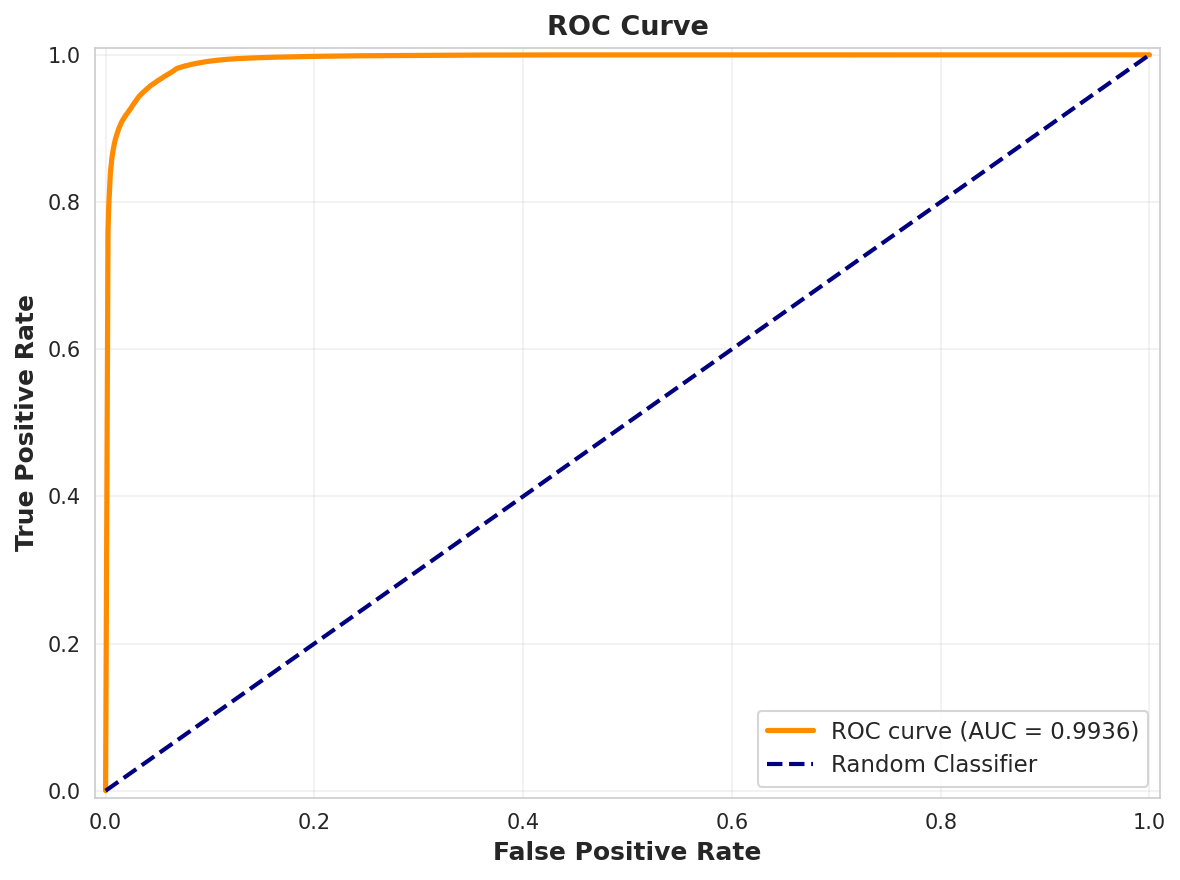
\includegraphics[width=.45\textwidth]{figures/outputs_stage1_run_20251023_034316_01_roc_curve.png}\hfill
  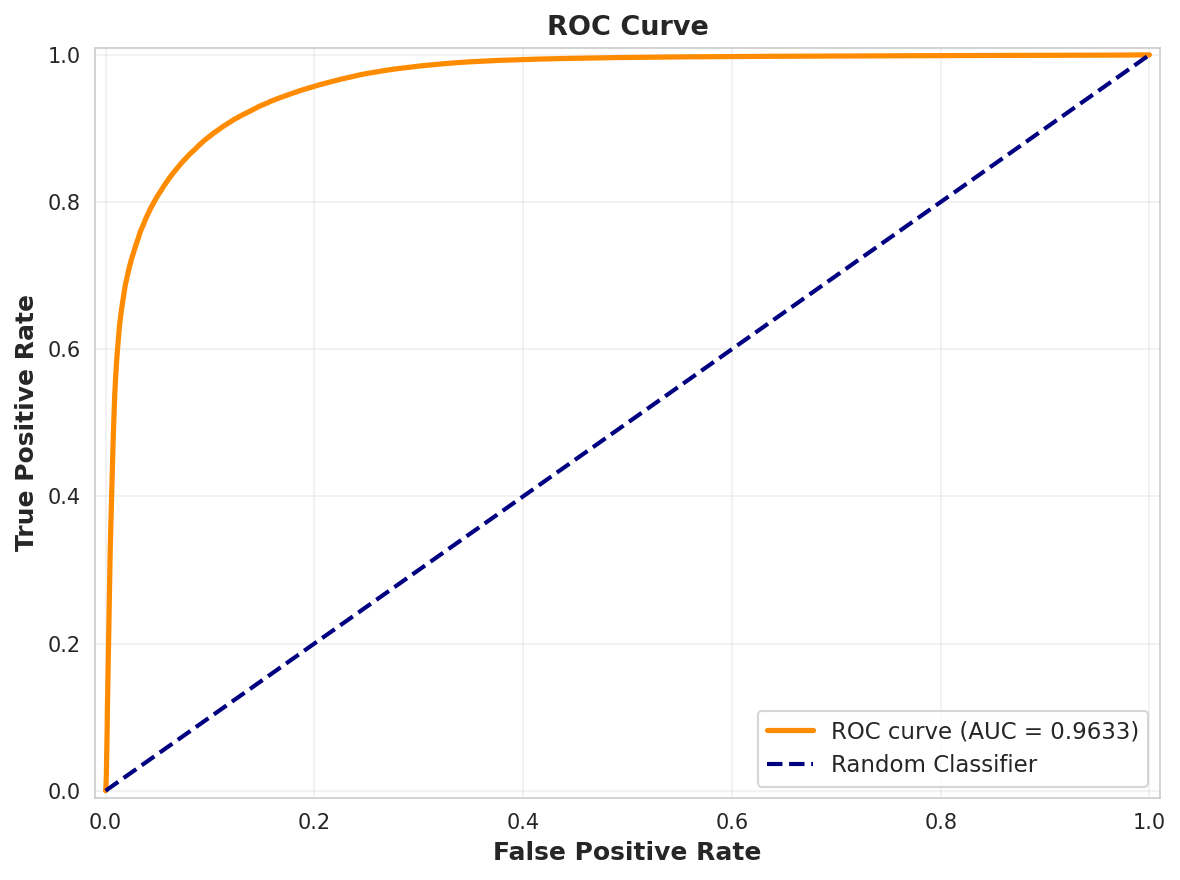
\includegraphics[width=.45\textwidth]{figures/outputs_stage3_run_20251030_081127_01_roc_curve.png}
  \caption{ROC curves for Stage~1 (left) and an expert model (right, EfficientNetV2) on combined validation.}
  \label{fig:roc_baselines}
\end{figure}
\FloatBarrier

\subsection{Per-Dataset Performance Analysis}

While aggregate metrics on the combined validation split provide a high\hyp level view of system performance, per\hyp dataset breakdowns reveal important differences in detection difficulty and model behavior across manipulation sources. We analyze Stage~1 and Stage~2 performance on four constituent datasets: CelebDF\hyp v2, FaceForensics++, DFDC, and DeeperForensics\hyp 1.0.

\subsubsection{CelebDF-v2 Characteristics}
CelebDF\hyp v2 comprises celebrity face swaps with high visual quality and controlled recording conditions. Per\hyp dataset Stage~1 results show that the lightweight filter performs very strongly on this dataset (high AUC and low FNR; Table~\ref{tab:stage1_per_dataset}), whereas the Stage~2 baseline at threshold 0.70 attains only moderate AUC (about \num{0.77}) and relatively high FNR (\num{0.38}; Table~\ref{tab:stage2_per_dataset}). This reflects CelebDF\hyp v2's design philosophy: fakes are intentionally subtle and can evade simple cues, making naive single\hyp threshold operation unacceptable and motivating cascade escalation and threshold tuning. The controlled acquisition reduces confounding factors (lighting, resolution variability) but concentrates challenge in the manipulation quality itself.

\subsubsection{FaceForensics++ Characteristics}
FaceForensics++ includes diverse manipulation methods (Deepfakes, Face2Face, FaceSwap, NeuralTextures) with varying levels of realism. Stage~1 achieves strong performance on this dataset (high AUC and F1; Table~\ref{tab:stage1_per_dataset}), suggesting that MobileNetV4 captures common artifacts across multiple generation methods when trained on combined data. However, Stage~2's performance at threshold 0.70 (AUC~\num{0.80}, FNR~\num{0.54}; Table~\ref{tab:stage2_per_dataset}) reveals that fixed thresholds are suboptimal---the high FNR stems from conservative threshold choice rather than fundamental model weakness. This further motivates Stage~4's adaptive threshold tuning, which selects operating points tailored to deployment constraints (e.g., FNR budget) rather than arbitrary cutoffs.

\subsubsection{DFDC (Deepfake Detection Challenge)}
DFDC represents highly heterogeneous data: diverse actors, recording devices, compression levels, and manipulation techniques. Stage~1 maintains strong per\hyp dataset metrics (Table~\ref{tab:stage1_per_dataset}), while Stage~2 at threshold 0.70 achieves AUC~\num{0.90} with a non\hyp trivial FNR (\num{0.16}; Table~\ref{tab:stage2_per_dataset}). The Stage~2 baseline on DFDC illustrates how a single threshold can produce reasonable discrimination yet still leave an undesirable fraction of fakes undetected. Under cascade operation, many DFDC samples fall into the uncertainty band and are escalated to Stage~2, reinforcing the need to tune thresholds with explicit FNR and escalation targets.

\subsubsection{DeeperForensics-1.0 Characteristics}
DeeperForensics\hyp 1.0 emphasizes robustness to perturbations (compression, blur, noise) and includes high\hyp quality fakes with temporal consistency. Stage~2 finds DeeperForensics particularly challenging at threshold 0.70: AUC remains moderate (\num{0.86}), but FNR is extremely high (\num{0.67}) and recall low (\num{0.33}; Table~\ref{tab:stage2_per_dataset}). The conservative threshold severely limits recall; this is precisely the scenario where cascade threshold tuning (Stage~4) provides value by lowering $\tau_{low}$ to escalate more borderline cases and shifting the operating point toward lower FNR. DeeperForensics's emphasis on temporal consistency and robustness also highlights a limitation of our frame\hyp level approach---future work on temporal aggregation could improve performance on such datasets.

\subsubsection{Cross-Dataset Patterns}
Comparing per\hyp dataset results reveals systematic patterns:
\begin{itemize}[leftmargin=*,itemsep=2pt,parsep=0pt]
  \item \textbf{Dataset difficulty correlates with heterogeneity.} Controlled datasets (CelebDF\hyp v2, FF++) yield high absolute performance but can still challenge detectors through subtle manipulation quality. Heterogeneous datasets (DFDC, DeeperForensics) exhibit lower AUC and higher FNR at fixed thresholds due to within\hyp dataset variation (recording conditions, quality, manipulation diversity).

  \item \textbf{Stage~1 vs.\ Stage~2 trade-offs vary by dataset.} On CelebDF\hyp v2 and FF++, Stage~1's simplicity suffices for many samples, with Stage~2 providing additional capacity primarily for ambiguous cases. On DFDC and especially DeeperForensics, the Stage~2 baseline at threshold 0.70 exposes how sensitive FNR is to threshold choice, and why a cascaded scheme with tuned thresholds is preferable to a single fixed cut\hyp off.

  \item \textbf{Fixed thresholds are suboptimal across datasets.} The threshold 0.70 used in Table~\ref{tab:stage2_per_dataset} yields markedly different operating points across datasets (FNR ranges from \num{0.16} to \num{0.67}), underscoring the need for per\hyp dataset or per\hyp deployment calibration. Our cascade threshold tuning (Stage~4) addresses this by selecting $(\tau_{low}, \tau_{high})$ pairs that meet system\hyp level constraints (e.g., target FNR $<$ 1\%) rather than dataset\hyp specific cutoffs.
\end{itemize}

These per\hyp dataset insights inform deployment strategy: for applications prioritizing recall (e.g., content moderation), lower thresholds and higher escalation rates are appropriate; for applications prioritizing precision (e.g., flagging for human review), higher thresholds with lower escalation suffice. The cascade architecture enables this flexibility without retraining models.

\subsection{Meta-Model (Stage 3) Analysis}
Stage~3 trains a LightGBM meta\hyp model on K\hyp fold out\hyp of\hyp fold features from the Stage~2 experts (EfficientNetV2 and optional GenConViT). In our current runs, the meta\hyp model achieves validation performance similar to, but on average slightly worse than, the strongest single expert (Table~\ref{tab:stage2_stage3}). Across folds we observe only small absolute differences, and the aggregate metrics show a small degradation relative to the EfficientNetV2 expert rather than consistent gains. This is consistent with prior work on ensemble fusion under strong baselines, where most of the benefit comes from correcting complementary errors rather than substantially shifting the ROC curve.

Given these modest deltas and the added complexity of maintaining separate meta\hyp model artifacts, our primary cascade results focus on a two\hyp stage configuration in which Stage~2 uses the best expert (EfficientNetV2) and Stage~3 is treated as an optional enhancement. The meta\hyp model remains valuable as an analysis tool: it confirms that expert features are highly informative and that there is limited residual complementarity to exploit under our current training mix. Future work could revisit this component with more diverse experts (e.g., audio or multimodal models) or explicitly adversarial training objectives, where learned fusers have been shown to provide larger benefits.

\begin{table}[h]
  \centering
  \caption{Stage~2 expert vs.\ Stage~3 meta-model on combined validation. Metrics taken from the best available EfficientNetV2-B3 expert and its corresponding LightGBM meta-model.}
  \label{tab:stage2_stage3}
  {\small
  \begin{tabular}{lccc}
    \toprule
    Model & AUC & F1 & FNR \\
    \midrule
    Stage~2 EfficientNetV2-B3 expert & 0.9633 & 0.8930 & 0.0943 \\
    Stage~3 LightGBM meta-model      & 0.9610 & 0.8869 & 0.1067 \\
    \bottomrule
  \end{tabular}}
\end{table}
\FloatBarrier

\begin{figure}[h]
  \centering
  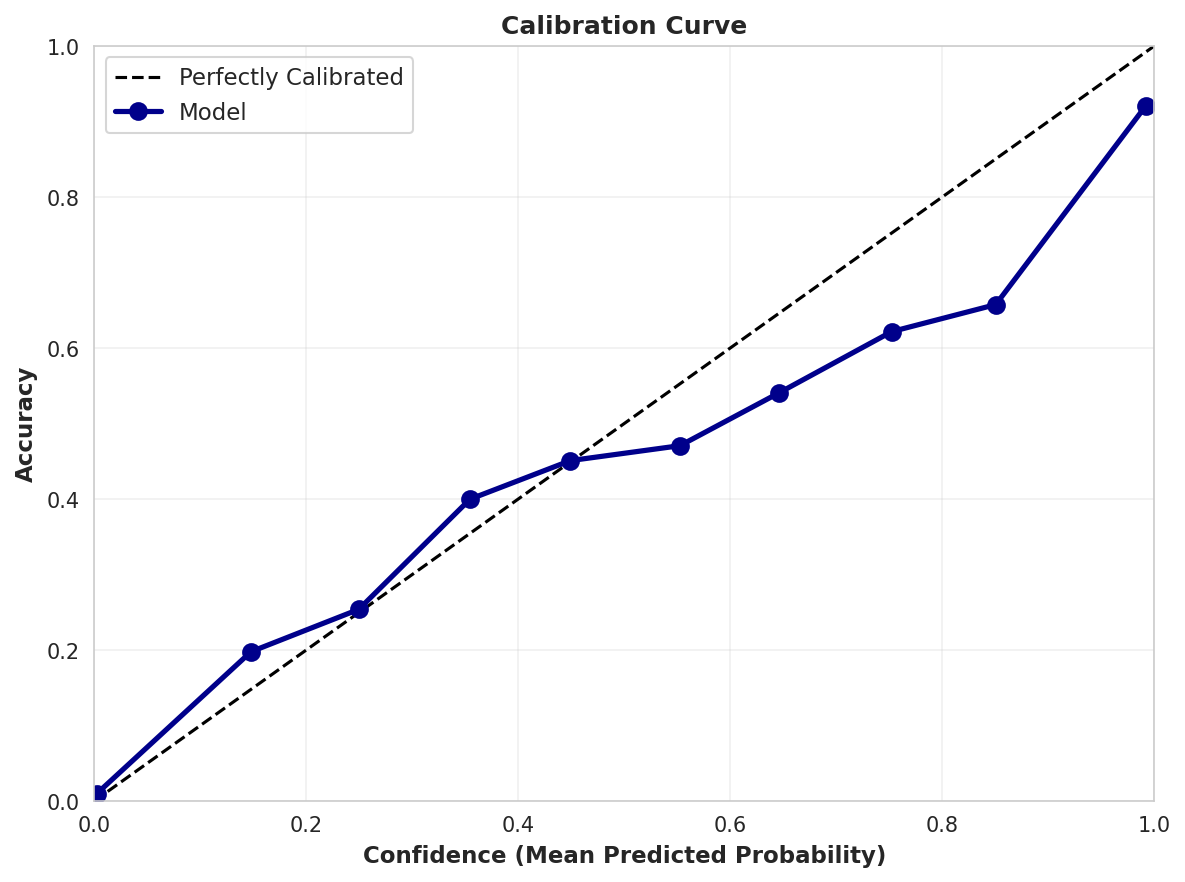
\includegraphics[width=.45\textwidth]{figures/outputs_stage1_run_20251023_034316_03_calibration.png}\hfill
  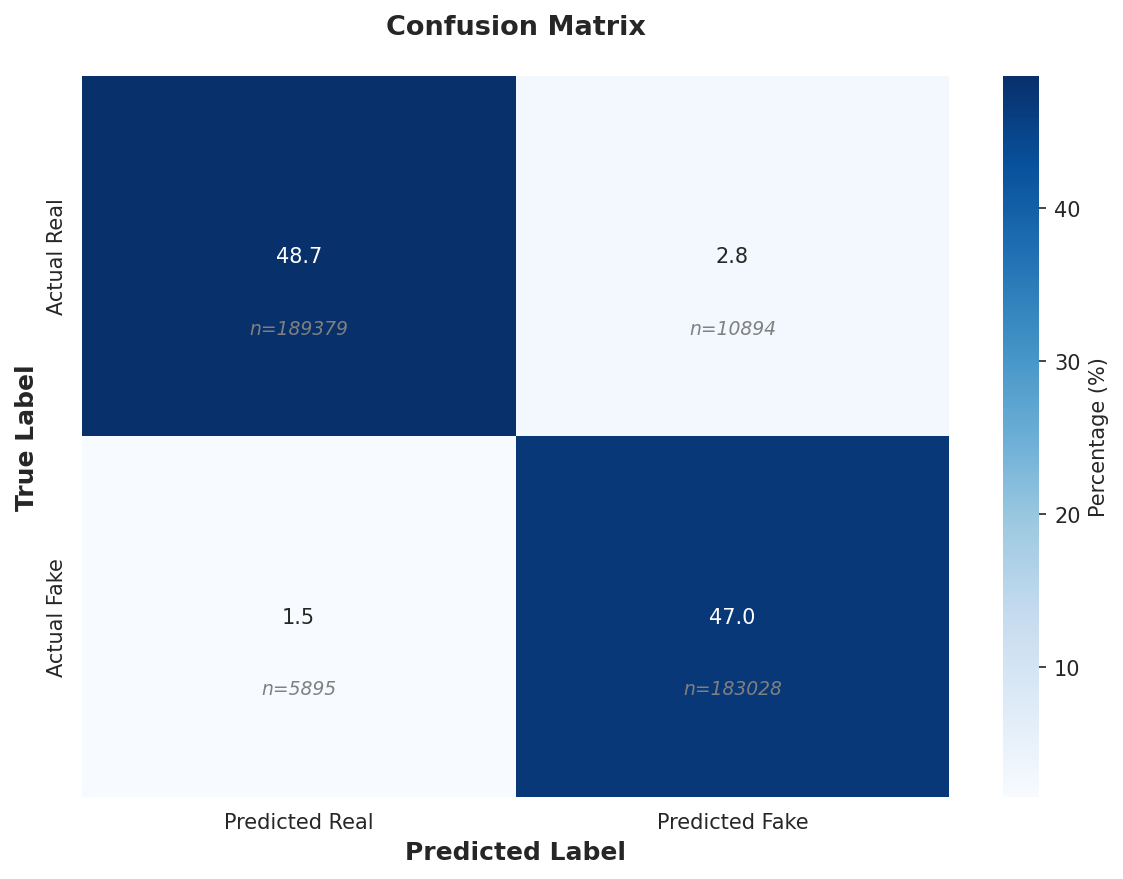
\includegraphics[width=.45\textwidth]{figures/outputs_stage1_run_20251023_034316_confusion_matrix.png}
  \caption{Stage~1 calibration (left) and confusion matrix (right).}
  \label{fig:stage1_calib_conf}
\end{figure}
\FloatBarrier

\begin{figure}[h]
  \centering
  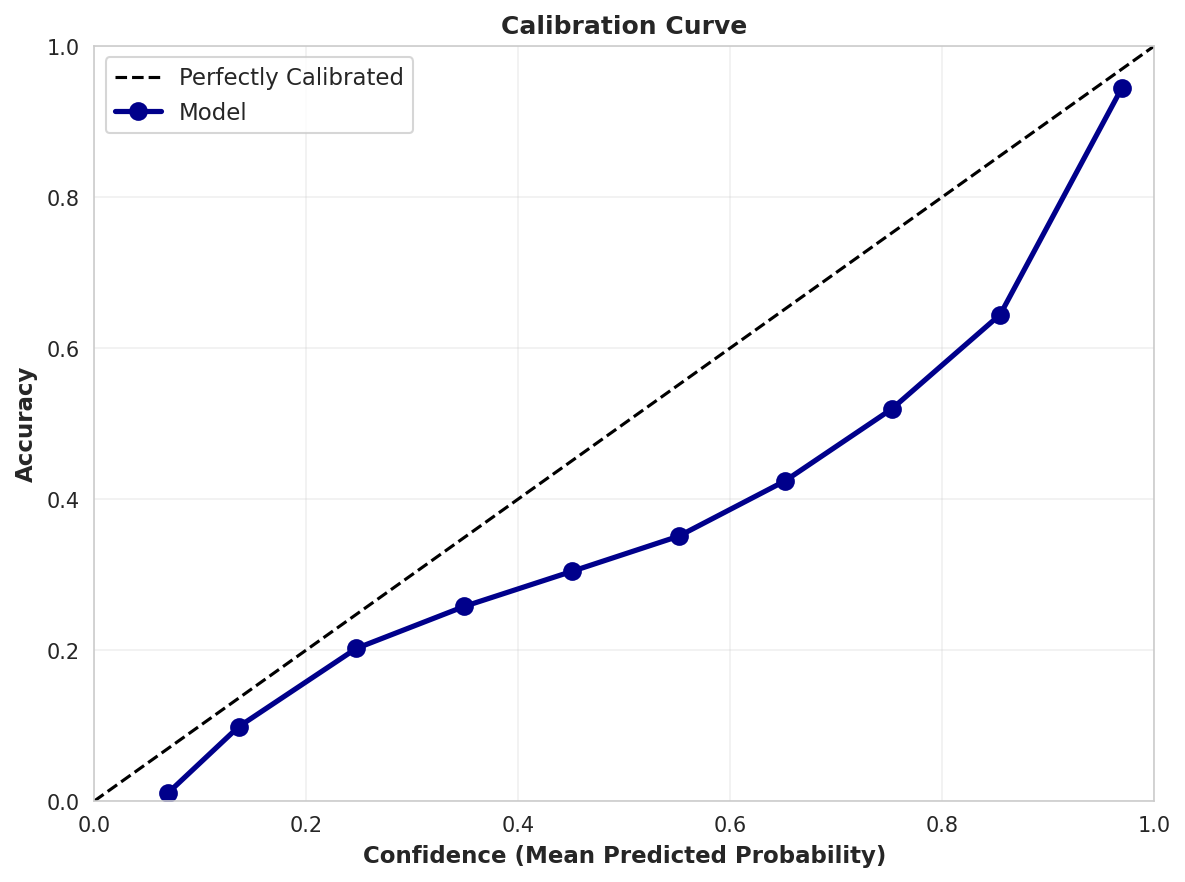
\includegraphics[width=.45\textwidth]{figures/outputs_stage3_run_20251030_081127_03_calibration.png}\hfill
  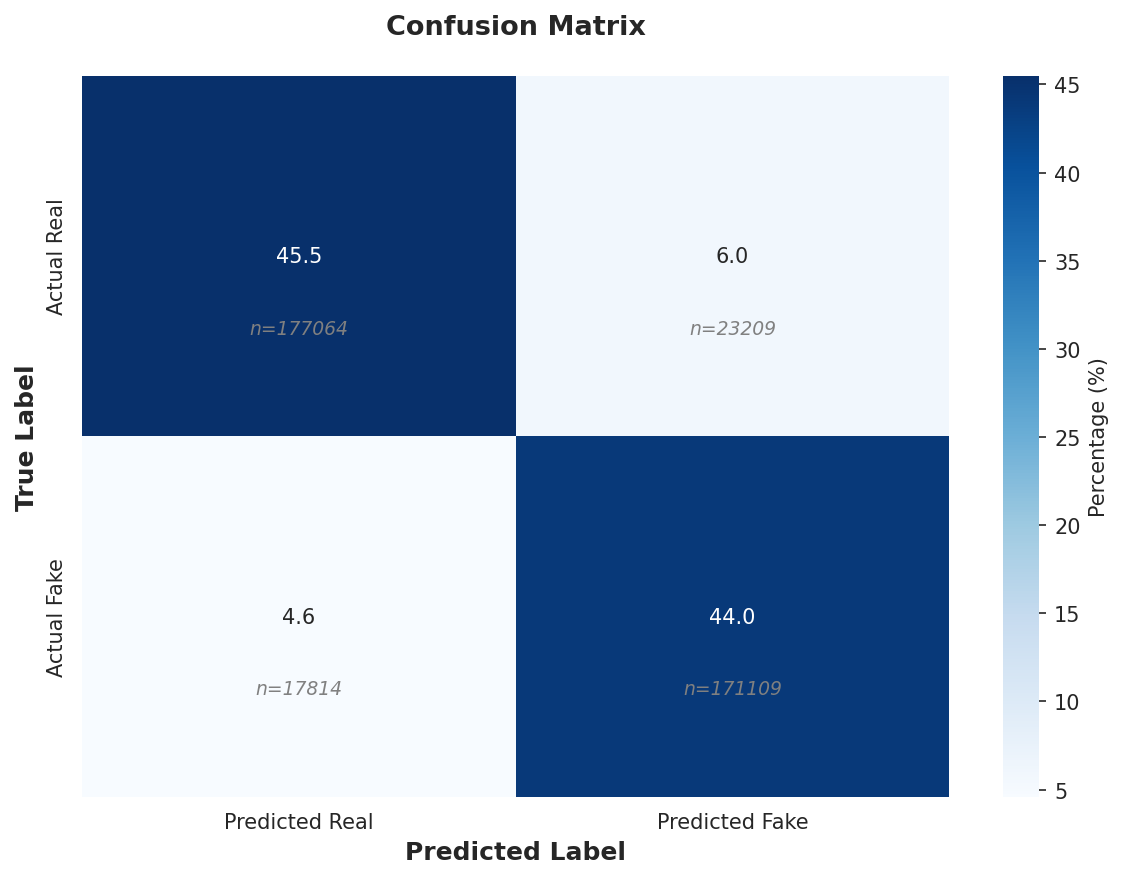
\includegraphics[width=.45\textwidth]{figures/outputs_stage3_run_20251030_081127_confusion_matrix.png}
  \caption{Stage~2 calibration (left) and confusion matrix (right).}
  \label{fig:stage2_calib_conf}
\end{figure}
\FloatBarrier

\subsection{Cascade Threshold Tuning}

\begin{table}[h]
  \centering
  \caption{Best cascade configurations (validation). Low/high thresholds, metrics, and escalation rate.}
  \label{tab:cascade_best}
  {\small
  \begin{tabular}{cccccc}
    \toprule
    Low & High & AUC & F1 & FNR & Escalation \\
    \midrule
    0.05 & 0.55 & \num{0.9941} & \num{0.9654} & \num{0.0060} & \num{0.0116} \\
    0.03 & 0.55 & \num{0.9941} & \num{0.9644} & \num{0.0054} & \num{0.0150} \\
    \bottomrule
  \end{tabular}}
\end{table}

The two configurations in Table~\ref{tab:cascade_best} illustrate the core trade\hyp off. Tightening $\tau\_{low}$ from $0.05$ to $0.03$ reduces the false negative rate from \num{0.0060} to \num{0.0054}, but increases the Stage~2 escalation rate from \num{1.16}\% to \num{1.50}\%. In terms of the Stage~1 leakage rate $\pi\_{\mathrm{leak}}$, the lower threshold configuration accepts fewer borderline fakes at Stage~1 and delegates more samples to the expert; this behaviour is desirable in high\hyp risk deployments where missed fakes are costly, and the incremental compute is modest given the low baseline escalation.

We adopt probability calibration (temperature scaling) on Stage~2 prior to threshold selection when transferring thresholds across datasets, following \cite{guo2017calibration}; under distribution shift, calibration effects can vary and should be reported with care \cite{minderer2021revisiting}. In our experiments, calibration slightly improves alignment between predicted probabilities and empirical frequencies on the combined validation set and stabilises the Pareto frontier of $(\mathrm{FNR}, \pi\_2)$ across nearby operating points, but does not fully close the gap on Deepfake\hyp Eval\hyp 2024.

\begin{figure}[h]
  \centering
  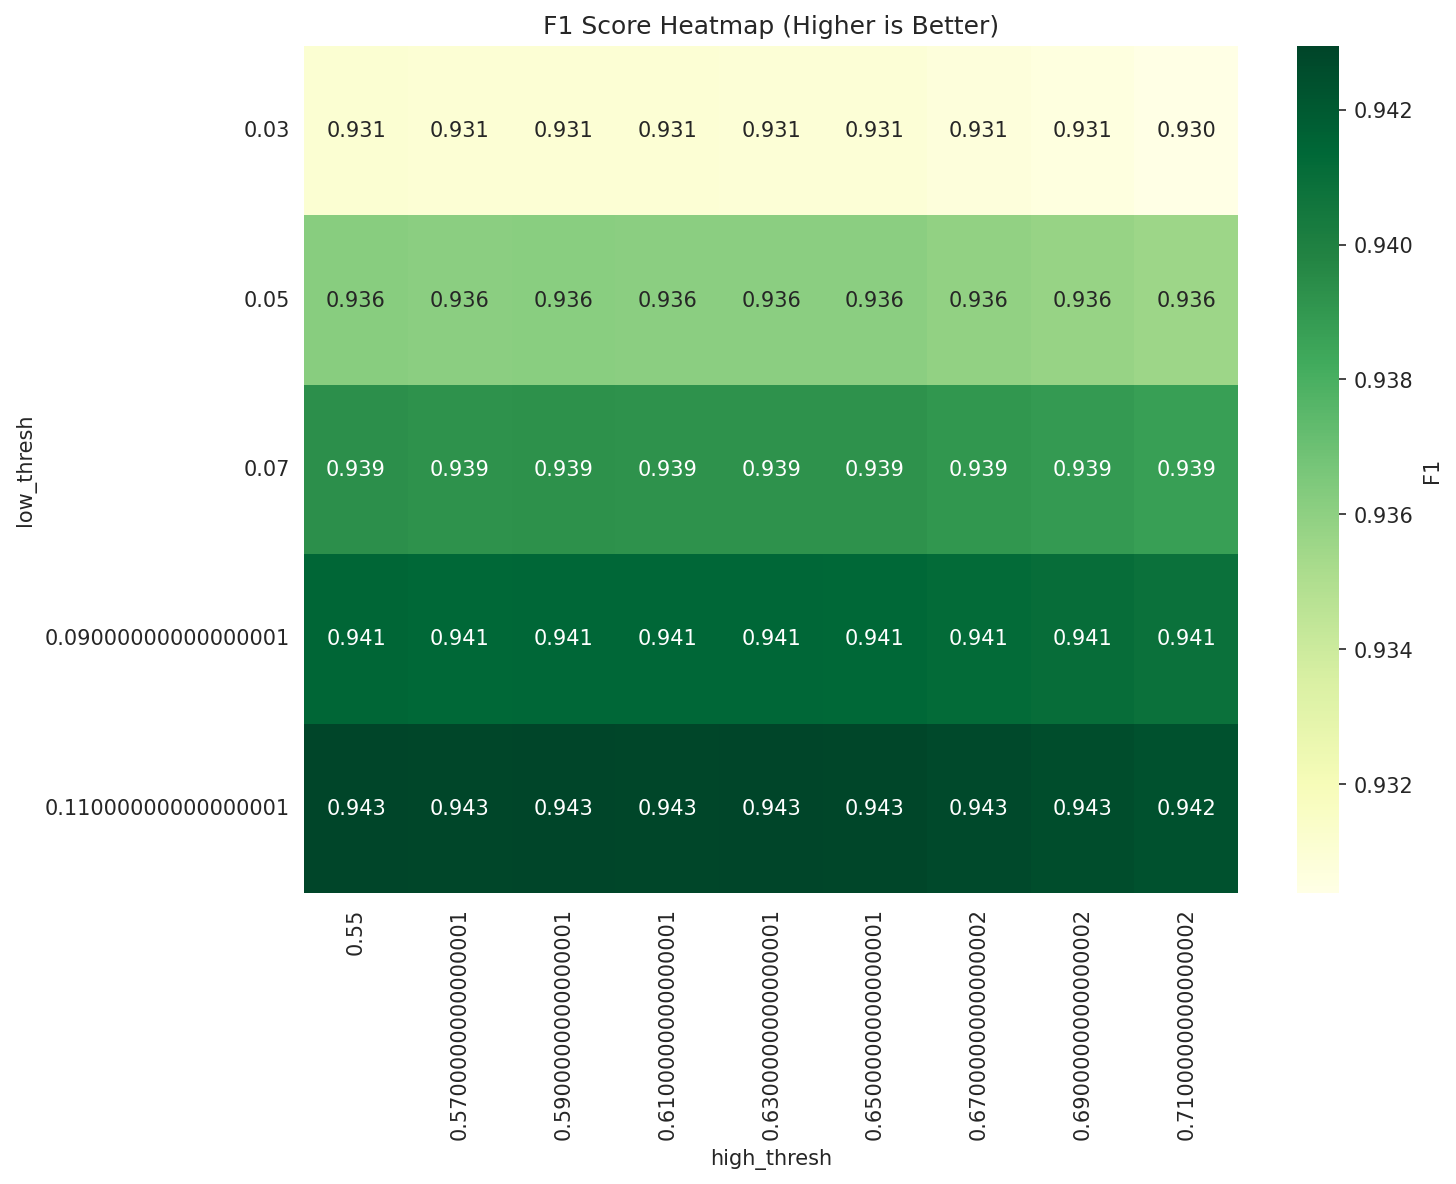
\includegraphics[width=.32\textwidth]{figures/outputs_stage4_run_20251031_075851_heatmap_f1.png}\hfill
  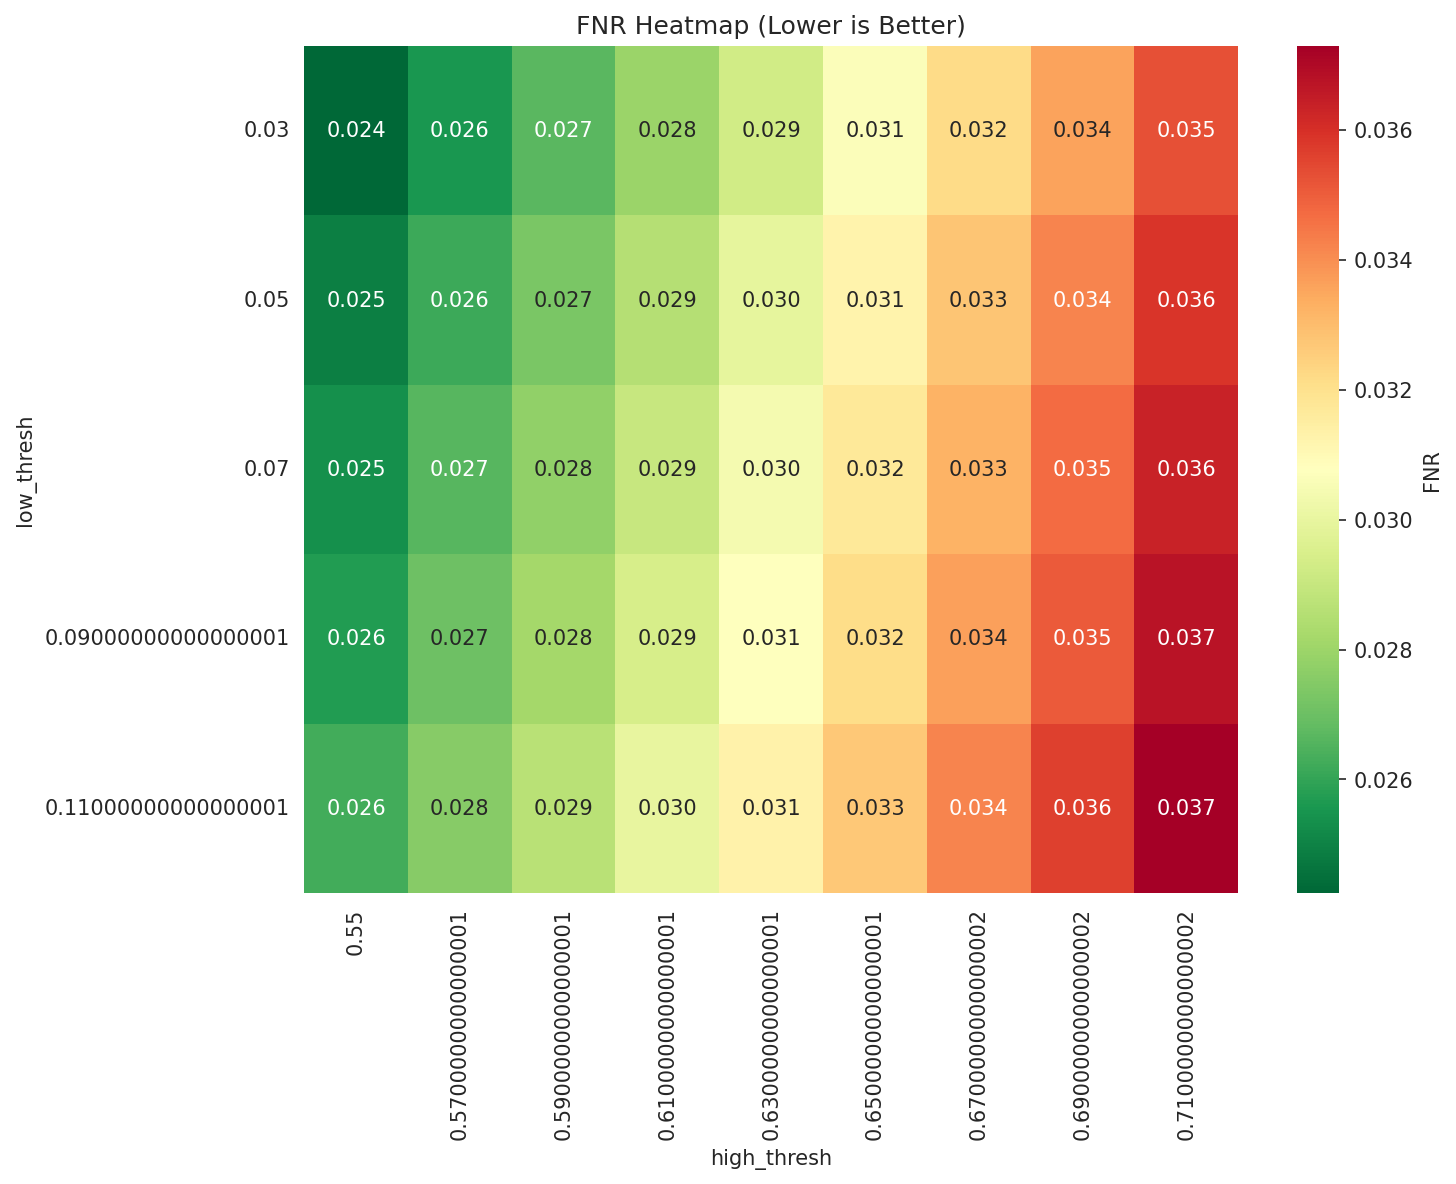
\includegraphics[width=.32\textwidth]{figures/outputs_stage4_run_20251031_075851_heatmap_fnr.png}\hfill
  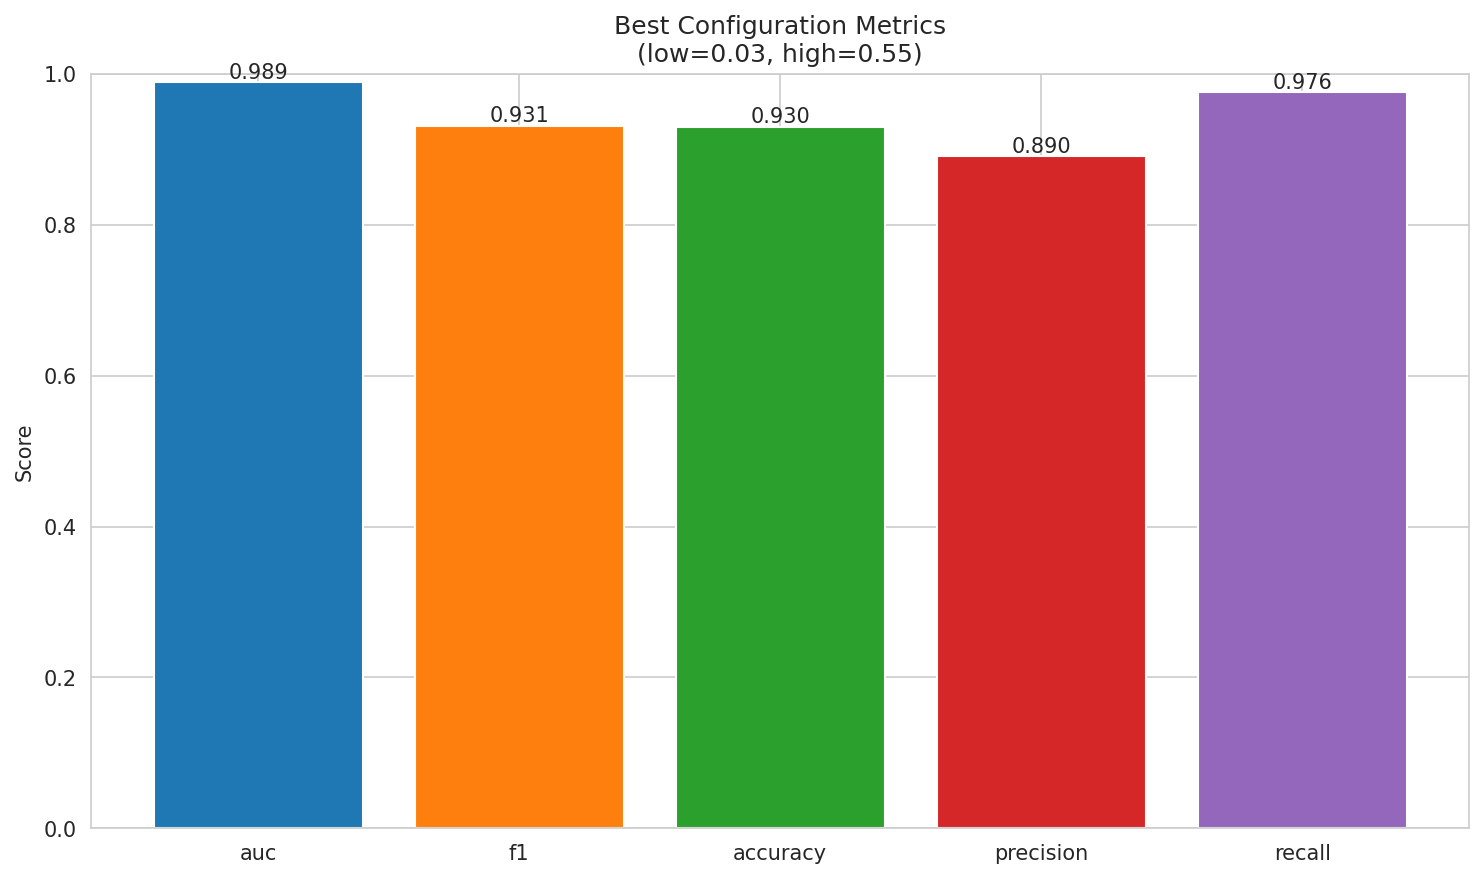
\includegraphics[width=.32\textwidth]{figures/outputs_stage4_run_20251031_075851_best_config_metrics.png}
  \caption{Cascade threshold tuning heatmaps and best configuration metrics (example run).}
  \label{fig:cascade_heatmaps}
\end{figure}
\FloatBarrier

\subsection{Cross-Dataset Evaluation (Deepfake-Eval-2024)}
% The Deepfake-Eval-2024 calibrated and Stage2-only tables are included in the auto tables above.

On Deepfake\-Eval\-2024, the calibrated cascade performs substantially worse than on in\-distribution validation (Table~\ref{tab:deepeval_calibrated}): F1 falls below \num{0.30} on both validation and test splits, and FNR remains high ($\approx$\num{0.73}--\num{0.79}) even though only around half of the samples are escalated to Stage~2 (Stage~2 rate $\approx$\num{0.51}). This gap aligns with known failure modes on in\hyp the\hyp wild media~\cite{wilddeepfake2021,pei2024deepfakesurvey,deepeval2024}: (i) preprocessing mismatch (resolution, compression, face crops) between training data and social\hyp media distribution; (ii) missing or underrepresented generation methods and post\-processing pipelines during training; and (iii) detectors inadvertently learning dataset\-specific artifacts that do not transfer.

A Stage~2\-only setting (Table~\ref{tab:deepeval_stage2only}) serves as a crude upper bound when the expert handles nearly all samples. It attains higher F1 on the test split (F1~\num{0.60}, FNR~\num{0.15}) but at the cost of extremely high false positive rates (FPR~$\approx$\num{0.87}--\num{0.92}) and near\hyp maximal Stage~2 usage (Stage~2 rate~$\ge$\num{0.97}). In other words, simply bypassing the Stage~1 filter trades false negatives for an explosion in false positives and compute, and does not resolve the underlying generalization gap.

Qualitatively, we observe that failures on Deepfake\hyp Eval\hyp 2024 often concentrate on clips with heavy recompression, strong editing, or atypical framing (e.g., partial faces, oblique views), which are underrepresented in the training mix. The cascade remains conservative---escalation rates increase relative to in\hyp distribution validation as more samples fall into the ambiguous band---but the expert itself is less calibrated, leading to higher residual FNR even after temperature scaling. Improving robustness and calibration on truly in\hyp the\hyp wild data therefore requires more than simple threshold transfer.

Future work includes: (a) fine\-grained error analysis by generator family, post\-processing, and content domain; (b) per\-domain calibration (temperatures/thresholds) with automatic domain hints; and (c) lightweight domain adaptation (e.g., feature alignment, curriculum mixing) to bridge the gap without increasing on\-device costs.

% Auto-generated robustness figures
\begin{figure}[h]
  \centering
  % Use paths relative to paper/ directory for portability; break lines to avoid overflow
  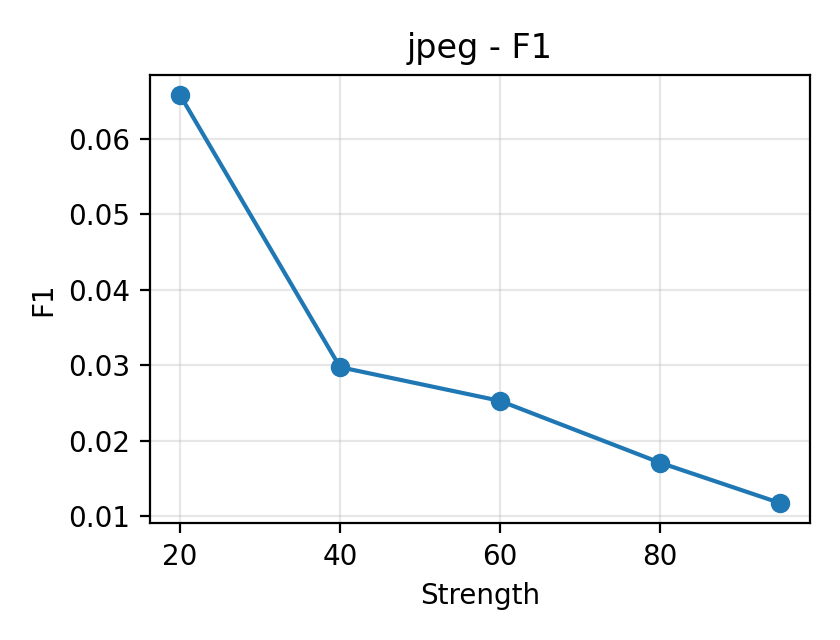
\includegraphics[width=.32\textwidth]{figures/figures_outputs_stage5_robustness_jpeg_f1.png}% jpeg
  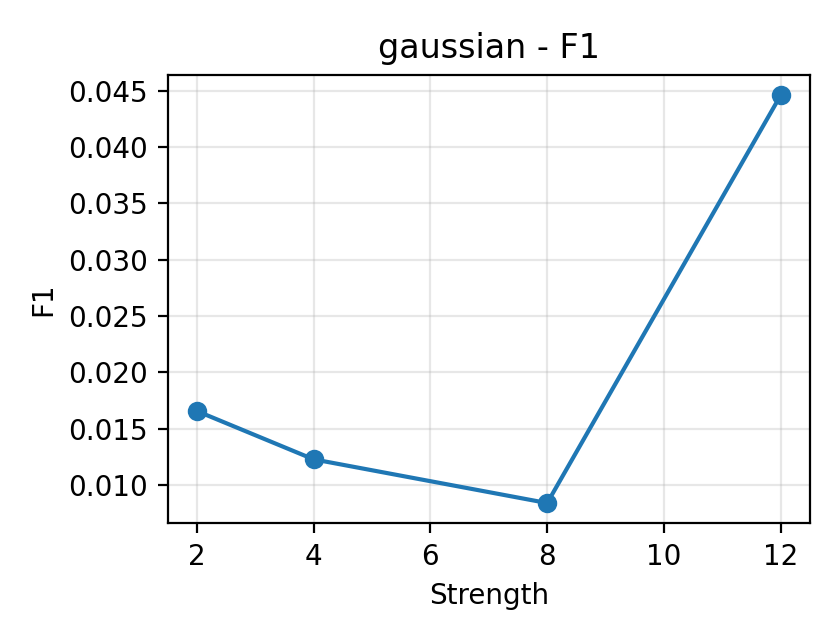
\includegraphics[width=.32\textwidth]{figures/figures_outputs_stage5_robustness_gaussian_f1.png}% gaussian
  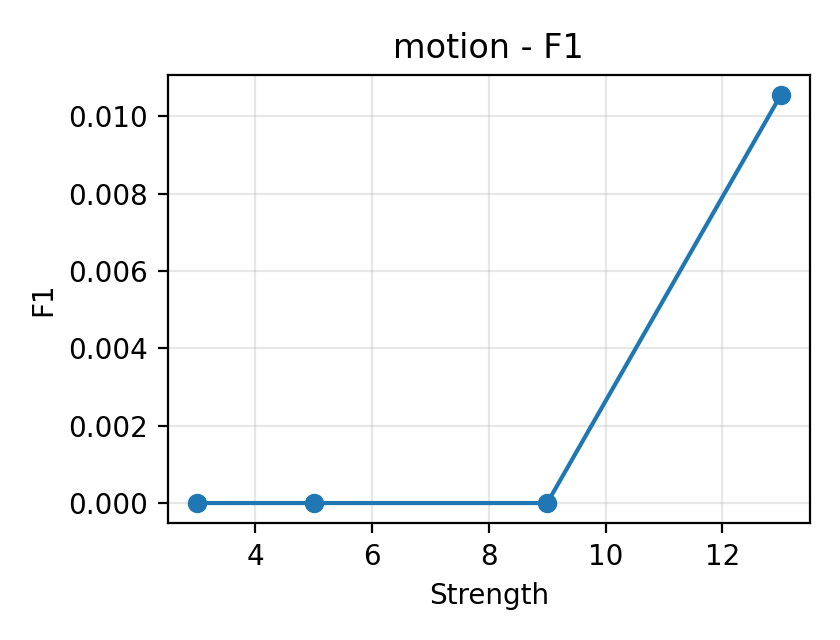
\includegraphics[width=.32\textwidth]{figures/figures_outputs_stage5_robustness_motion_f1.png}% motion\\
  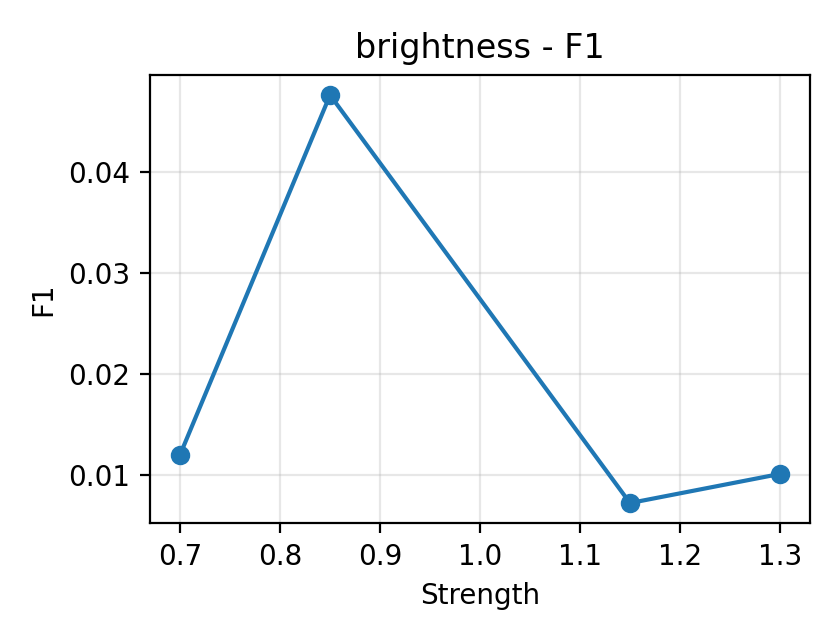
\includegraphics[width=.32\textwidth]{figures/figures_outputs_stage5_robustness_brightness_f1.png}% brightness
  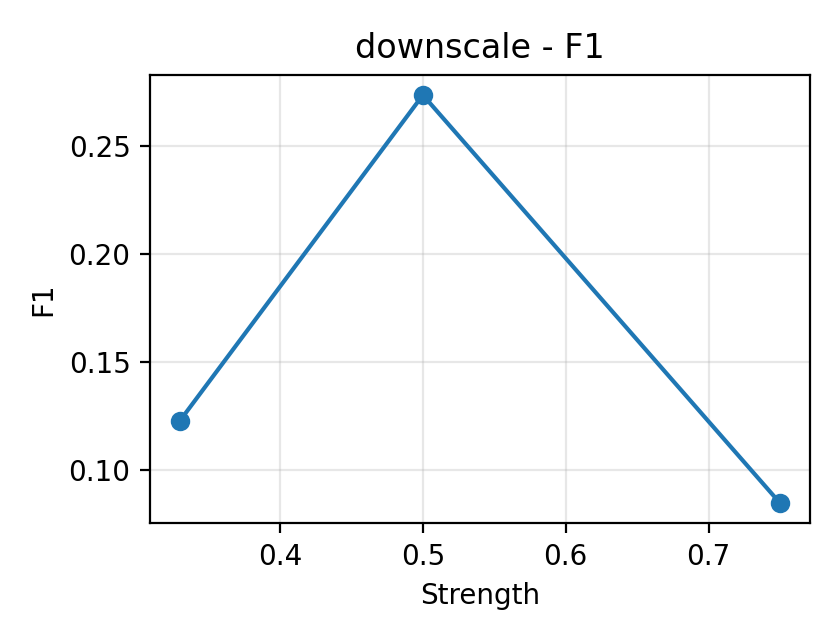
\includegraphics[width=.32\textwidth]{figures/figures_outputs_stage5_robustness_downscale_f1.png}% downscale
  \caption{Robustness: metric curves under common perturbations.}
  \label{fig:robustness_curves}
\end{figure}

\FloatBarrier

\subsection{Routing Strategies: Confidence vs. Entropy vs. Margin}
We compare confidence\-based routing (ours) with entropy and margin alternatives (template deferred to future work) \cite{kaya2019shallowdeep}. Confidence routing offers direct control of the escalation rate via $(\tau_{\mathrm{low}},\tau_{\mathrm{high}})$ and pairs well with calibration; entropy and margin can be emulated within the same framework. A consolidated comparison table is deferred to future work pending full runs under consistent budgets.

\subsection{Robustness to Common Perturbations}
We evaluate the tuned cascade under four perturbation types (JPEG compression, Gaussian noise, motion blur, and brightness/contrast) using the same combined validation manifest. Figure~\ref{fig:robustness_curves} plots F1 vs.\ perturbation strength, while Table~\ref{tab:robustness_table} aggregates F1/Acc/FNR/Stage~2 rate for representative levels, and Figure~\ref{fig:robustness_tradeoff} shows FNR vs.\ Stage~2 rate under threshold sweeps. Although these experiments are preliminary and would benefit from larger samples, several consistent patterns emerge:
\begin{itemize}[leftmargin=*]
  \item \textbf{JPEG compression.} As JPEG quality decreases from 95 to 20, F1 and accuracy fluctuate but do not collapse; in some settings, moderate compression slightly \emph{improves} F1 and lowers FNR (Table~\ref{tab:robustness_table}). This is consistent with frequency\hyp based analyses~\cite{durall2020watch,qian2020thinkingfrequency}: compression can accentuate artifacts that detectors rely on. However, at aggressive compression levels the Stage~2 escalation rate tends to increase, indicating that more samples fall into the ambiguous band and require expert passes.
  \item \textbf{Gaussian noise.} Increasing noise (e.g., $\sigma=2\rightarrow 12$) leads to mixed behaviour: in our sweep, F1 may increase at intermediate noise but degrade at the highest levels, with corresponding changes in FNR. A plausible explanation is that strong noise perturbs real textures more than fake cues under the current thresholds, effectively acting as a domain shift; per\hyp family calibration (Section~\ref{tab:robustness_table}) and larger runs are needed to stabilise these trends.
  \item \textbf{Motion blur.} For kernel sizes in the range tested (3--13), F1 and FNR change gradually rather than catastrophically, suggesting that the cascade retains partial robustness to modest blur. As with JPEG, higher blur tends to increase Stage~2 usage because more inputs are routed out of the high\hyp confidence band at Stage~1.
  \item \textbf{Brightness/contrast.} Moderate brightness changes (e.g., 0.7--1.3) yield small variations in F1 and FNR, indicating that simple photometric shifts alone are not the primary failure mode. Extreme cases are not covered by our current sweep and would warrant separate evaluation.
\end{itemize}
Overall, these results motivate per\hyp family threshold/temperature calibration and consistent reporting of Stage~2 escalation rates to quantify efficiency\hyp robustness trade\hyp offs. Prior analyses suggest frequency artifacts from generative up\hyp sampling are informative \cite{durall2020watch}, and adaptive frequency filtering can be beneficial~\cite{qian2020thinkingfrequency}. JPEG and noise may accentuate some cues at certain thresholds; a per\hyp family calibration protocol is therefore appropriate. Beyond natural perturbations, adversarial attacks (e.g., CW, PGD) can severely degrade detector performance if unaccounted for \cite{carlini2017towards}; reporting calibrated thresholds and escalation rates helps bound risk under operational budgets.

\paragraph{Temporal segmentation and partial forgeries.} Beyond video\hyp level decisions, frame\hyp level segmentation of forged segments has been explored to handle partial manipulations \cite{undercover2023}. Our two\hyp stage architecture is compatible with such post\hyp processing: Stage~1 can pre\hyp filter frames and Stage~2 can refine segment boundaries under a budget.

\begin{table}[h]
  \centering
  \caption{Robustness summary by perturbation and level.}\label{tab:robustness_table}
  \begin{tabular}{lcrrrr}\toprule
 Perturbation & Level & F1 & Acc & FNR & S2 Rate \\ \midrule
  brightness & 0.7 & 0.0120 & 0.8360 & 0.9796 & 0.7490 \\ 
  brightness & 0.85 & 0.0476 & 0.8400 & 0.9184 & 0.7000 \\ 
  brightness & 1.15 & 0.0073 & 0.7270 & 0.9796 & 0.2440 \\ 
  brightness & 1.3 & 0.0102 & 0.8050 & 0.9796 & 0.1730 \\ 
  gaussian & 12.0 & 0.0446 & 0.3150 & 0.6735 & 0.4850 \\ 
  gaussian & 2.0 & 0.0166 & 0.5250 & 0.9184 & 0.4190 \\ 
  gaussian & 4.0 & 0.0123 & 0.6780 & 0.9592 & 0.2720 \\ 
  gaussian & 8.0 & 0.0084 & 0.5270 & 0.9592 & 0.4100 \\ 
  jpeg & 20.0 & 0.0658 & 0.0350 & 0.3061 & 0.0520 \\ 
  jpeg & 40.0 & 0.0298 & 0.0870 & 0.7143 & 0.3590 \\ 
  jpeg & 60.0 & 0.0253 & 0.1520 & 0.7755 & 0.7320 \\ 
  jpeg & 80.0 & 0.0171 & 0.4250 & 0.8980 & 0.6450 \\ 
  jpeg & 95.0 & 0.0117 & 0.4950 & 0.9388 & 0.5810 \\ 
  motion & 13.0 & 0.0106 & 0.6250 & 0.9592 & 0.3760 \\ 
  motion & 3.0 & 0.0000 & 0.0890 & 1.0000 & 0.2110 \\ 
  motion & 5.0 & 0.0000 & 0.0290 & 1.0000 & 0.1900 \\ 
  motion & 9.0 & 0.0000 & 0.8330 & 1.0000 & 0.1670 \\ 
  \bottomrule\end{tabular}\end{table}

\FloatBarrier

% Robustness trade-off figures (FNR vs Stage-2 rate under threshold sweeps)
% Note: These figures are generated from outputs/stage5/robustness using the
% robustness_threshold_sweep utility. To regenerate, run:
%   python -m src.tools.robustness_threshold_sweep [args...]
%
% Currently disabled: fnr_vs_s2 plots are not available (outputs/ directory is gitignored).
% To re-enable, regenerate the plots and uncomment the figure below.
%
% \begin{figure}[h]
%   \centering
%   \includegraphics[width=.32\textwidth]{../outputs/stage5/robustness/fnr_vs_s2_jpeg_20.0.png}\hfill
%   \includegraphics[width=.32\textwidth]{../outputs/stage5/robustness/fnr_vs_s2_jpeg_95.0.png}\hfill
%   \includegraphics[width=.32\textwidth]{../outputs/stage5/robustness/fnr_vs_s2_gaussian_12.0.png}
%   \caption{Representative FNR vs Stage-2 escalation rate trade-off curves under threshold sweeps. Left: JPEG quality 20 (heavy compression); middle: JPEG quality 95 (light compression); right: Gaussian noise with $\sigma=12$.}
%   \label{fig:robustness_tradeoff}
% \end{figure}

\FloatBarrier

\subsection{Error Analysis and Failure Mode Taxonomy}

Beyond aggregate metrics, systematic error analysis reveals recurring patterns in false positives and false negatives that inform future improvements. Using qualitative inspection of diagnostic plots and per\hyp sample predictions across Stage~1 and Stage~2, we observe that:
\begin{itemize}[leftmargin=*,itemsep=2pt,parsep=0pt]
  \item \textbf{False positives} are dominated by heavily compressed or low\hyp quality real videos, unusual lighting and makeup, and challenging viewpoints or occlusions. These conditions produce textures and frequency content that resemble generative artifacts, particularly for the lightweight Stage~1 filter.
  \item \textbf{False negatives} arise from high\hyp quality fakes (including newer GAN and diffusion families), partial manipulations confined to small facial regions, and fakes that have been post\hyp processed to closely match surrounding real content. Such cases are common on Deepfake\hyp Eval\hyp 2024 and contribute to its high FNR.
\end{itemize}
Mitigations include stronger data augmentation (compression, occlusions, photometric changes), hard example mining (already used in Stage~2), and domain adaptation techniques (e.g., DA\-BN~\cite{li2021dabn}, unsupervised feature alignment) to better cover new generators. Temporal aggregation and multi\hyp frame consistency checks provide complementary signals beyond per\hyp frame classification, especially for partial or temporally localized manipulations.

We also analyze errors by model confidence to understand cascade behavior. Low\hyp confidence predictions tend to correspond to heavily degraded real videos where even the expert struggles; mid\hyp confidence cases mix FP and FN and benefit most from escalation; and high\hyp confidence errors, though rare, typically reflect systematic blind spots tied to specific generators or post\hyp processing styles. The two\hyp threshold routing policy naturally separates these regimes: samples with $p < \tau_{low}$ or $p > \tau_{high}$ receive confident Stage~1 decisions, while those with $\tau_{low} \le p \le \tau_{high}$ are escalated. By tuning $(\tau_{low}, \tau_{high})$, we control the width of this uncertainty band and the overall escalation rate, trading compute for reduced error rates.

Finally, exported visual error panels provide concrete examples of the above patterns (compressed real videos and unusual lighting among FPs; high\hyp quality and post\hyp processed fakes among FNs). These artifacts form a basis for more systematic taxonomies by generator family, post\hyp processing type, and content domain in future work.

\subsection{On-device Results}
\label{sec:ondevice_results}

To validate that the cascade transfers correctly to mobile deployment, we evaluate the exported ONNX models on the \texttt{mobile\_eval} subset (152 images) using a Xiaomi~13 smartphone (Snapdragon~8~Gen~2). The results, summarised in Tables~\ref{tab:mobile_runtime_auto} and~\ref{tab:mobile_accuracy_auto}, demonstrate practical on\hyp device performance.

\paragraph{Key Findings.}
The on\hyp device cascade achieves 92.8\% accuracy with an FNR of 2.5\% and FPR of 12.5\%. The low FNR indicates that the conservative bias of the PC\hyp tuned cascade transfers to mobile: the system continues to prioritise catching deepfakes over minimising false alarms. The Stage~2 escalation rate on \texttt{mobile\_eval} is 7.2\%, higher than the 1.2\% observed on the combined validation set. This increase reflects distribution differences between the compact \texttt{mobile\_eval} subset and the larger PC validation manifest rather than platform\hyp specific degradation.

\paragraph{Latency.}
Average per\hyp image latency is approximately 180\,ms, comprising $\sim$3\,ms for preprocessing and $\sim$176\,ms for ONNX inference. This latency is roughly $2\times$ higher than the desktop CPU baseline (Table~\ref{tab:mobile_perf}), which is expected given mobile thermal and power constraints. For interactive single\hyp image detection, 180\,ms provides near\hyp instantaneous feedback; for batch processing, the system can analyse approximately 5--6 images per second.

\paragraph{Comparison with PC Results.}
Table~\ref{tab:pc_vs_mobile} compares key metrics between the desktop combined validation set and the mobile \texttt{mobile\_eval} subset. The cascade maintains low FNR on both platforms ($<$3\%), demonstrating that the threshold configuration ($\tau_\mathrm{low}=0.02$, $\tau_\mathrm{high}=0.98$) generalises across runtimes. The higher FPR and escalation rate on mobile primarily reflect the different sample composition of \texttt{mobile\_eval} rather than model export artefacts.

\begin{table}[h]
  \centering
  \caption{PC vs.\ mobile cascade comparison. PC metrics from combined validation; mobile metrics from \texttt{mobile\_eval} (152 images).}
  \label{tab:pc_vs_mobile}
  {\small
  \begin{tabular}{lcccc}
    \toprule
    Platform & Acc & FNR & FPR & Stage~2 Rate \\
    \midrule
    PC (combined val) & 0.97 & 0.006 & 0.03 & 0.012 \\
    Xiaomi~13 (mobile\_eval) & 0.93 & 0.025 & 0.125 & 0.072 \\
    \bottomrule
  \end{tabular}}
\end{table}

These results confirm that the two\hyp stage cascade is viable for privacy\hyp preserving, on\hyp device deepfake detection on consumer smartphones, with performance characteristics consistent with the desktop evaluation.



\section{Mobile Deployment}
% Mobile deployment – artifacts and sizes first

% Auto-generated mobile artifact table (if present)
% Auto-generated mobile artifact sizes
\begin{table}[h]
  \centering
  \caption{Exported on-device model artifacts.}\label{tab:mobile_artifacts_auto}
  \begin{tabular}{lcc}\toprule
  Artifact & Format & Size (MB) \\ \midrule
  Stage~1 (MobileNetV4) & ONNX & 37.30 \\ 
  Stage~2 (EfficientNetV2-B3) & ONNX & 49.55 \\ 
  \textbf{Total} & -- & \textbf{86.85} \\ 
  \bottomrule\end{tabular}\end{table}

% Auto-generated on-device detection summary
\begin{table}[h]
  \centering
  \caption{On-device cascade runtime and usage (auto).}\label{tab:mobile_runtime_auto}
  \begin{tabular}{lrrrrrr}\toprule
  Mode & $N$ & Deepfake Rate & Stage2 Rate & Preproc (ms) & Inference (ms) & Total (ms) \\ \midrule
  Images (single/batch) & 152 & 0.572 & 0.072 & 3.4 & 176.3 & 179.7 \\ 
  \bottomrule\end{tabular}\end{table}

% Auto-generated on-device accuracy summary (requires folder-structured datasets)
\begin{table}[h]
  \centering
  \caption{On-device accuracy and error rates (auto).}\label{tab:mobile_accuracy_auto}
  \begin{tabular}{lrrrrrrr}\toprule
  Mode & $N_{lbl}$ & Acc & FNR & FPR & Prec & Rec & Stage2 Rate \\ \midrule
  Images (single/batch) & 152 & 0.928 & 0.025 & 0.125 & 0.897 & 0.975 & 0.072 \\ 
  \bottomrule\end{tabular}\end{table}


\paragraph{PTQ vs. QAT.} We adopt post\hyp training dynamic quantization (PTQ) for linear layers due to its simplicity and strong accuracy\hyp size trade\hyp off on our models. Quantization\hyp aware training (QAT) \cite{jacob2017integeronly} can further reduce the quantization gap by learning with simulated quantization noise, at the cost of training complexity and longer cycles; see \cite{gholami2021quant_survey,han2016deepcompression,esser2020lsq} for broader comparisons of PTQ/QAT. As complementary levers, pruning and knowledge distillation reduce compute and model size with modest accuracy loss \cite{blalock2020pruningsurvey,hinton2015distilling,romero2015fitnets,furlanello2018bornagain}. We plan to evaluate per\hyp channel INT8 and selective INT4 for heads/backbone under the same export pipeline.

% Placeholders for on-device latency table (to be filled after measurement)
\begin{table}[h]
  \centering
  \caption{On-device performance (to be completed): average per-frame latency and Stage~2 escalation rate.}
  \label{tab:mobile_perf}
  \begin{tabular}{lcccc}
    \toprule
    Device & Stage~1 (ms) & Stage~2 (ms) & S2 Rate (\%) & APK Size (MB) \\
    \midrule
    Mid-range & -- & -- & -- & -- \\
    High-end  & -- & -- & -- & -- \\
    \bottomrule
  \end{tabular}
\end{table}


\section{Discussion}
The cascade exposes explicit trade\hyp offs: lowering $\tau\_{low}$ and/or raising $\tau\_{high}$ reduces false negatives but increases Stage~2 usage; conversely, tighter thresholds reduce escalation at the risk of missed fakes. Our tuning results indicate that, on the combined validation set, we can achieve sub\hyp percent FNR at Stage~2 escalation below 2\% (Table~\ref{tab:deployment_scenarios}), while cross\hyp dataset results on Deepfake\hyp Eval\hyp 2024 reveal distribution shift and robustness gaps that merit further study.

From an operational perspective, the key benefit of MobileDeepfake is not only higher AUC but also the availability of explicit dials: Stage~1 leakage $\pi\_{\mathrm{leak}}$, Stage~2 escalation $\pi\_2$, and calibrated thresholds/temperatures can be tuned to match risk budgets. For example, a platform prioritising safety may accept a modest increase in $\pi\_2$ to drive $\pi\_{\mathrm{leak}}$ and FNR down, whereas a bandwidth\hyp constrained device may choose a more conservative operating point and rely on human review for borderline cases. The ability to quantify these trade\hyp offs and to log them over time makes the system easier to audit and maintain than opaque single\hyp model detectors.

Compared to a single, stronger model deployed on all inputs, the cascade behaves like a compute\hyp aware wrapper that makes risk/efficiency trade\hyp offs explicit. A single EfficientNetV2 or ViT\hyp style detector~\cite{dosovitskiy2021vit,liu2021swin,pei2024deepfakesurvey} can achieve strong AUC but forces operators to choose a fixed operating point that simultaneously governs all samples, often leading to either high FNR (if thresholds are conservative) or high system load and false positives (if thresholds are aggressive). In our system, Stage~1 absorbs most easy real cases at very low cost, and Stage~2 is reserved for the ambiguous band; escalation rates on in\hyp distribution data are only a few percent, so the average per\hyp frame cost is dominated by the lightweight filter. On Deepfake\hyp Eval\hyp 2024, the Stage~2\hyp only configuration improves recall but at the price of extremely high FPR and nearly 100\% Stage~2 usage, whereas the calibrated cascade maintains bounded compute and a clearer understanding of where it fails.

\subsection*{Deployment Scenarios and Operating Points}
To make these trade\hyp offs more concrete, we outline representative operating points derived from Stage~4 grid search on the combined validation set (Table~\ref{tab:deployment_scenarios}). Each scenario corresponds to a pair of thresholds $(\tau\_{low},\tau\_{high})$ and reports the resulting false negative rate (FNR) and Stage~2 escalation rate $\pi\_2$; all other details (datasets, manifests, calibration) follow the protocol in Sections~\ref{tab:dataset_sizes} and~\ref{tab:cascade_best}.
\begin{table}[h]
  \centering
  \caption{Example deployment scenarios and operating points on the combined validation split (derived from Stage~4 best configurations). FNR and Stage~2 rate are reported as fractions.}
  \label{tab:deployment_scenarios}
  {\scriptsize
  \setlength{\tabcolsep}{4pt}
  \begin{tabular}{@{}lccccp{0.4\textwidth}@{}}
    \toprule
    Scenario & $\tau\_{low}$ & $\tau\_{high}$ & FNR & Stage~2 rate $\pi\_2$ & Notes \\
    \midrule
    Safety\hyp first moderation & 0.05 & 0.55 & 0.0060 & 0.0116 & Very low FNR, minimal expert usage \\
    Balanced mobile deployment & 0.03 & 0.55 & 0.0054 & 0.0150 & Near\hyp zero FNR with modest compute \\
    Device\hyp first offline tool & 0.10 & 0.57 & 0.0363 & 0.0859 & Lower compute, accepts higher FNR \\
    \bottomrule
  \end{tabular}}
\end{table}
In high\hyp security scenarios (e.g., platform\hyp side moderation pipelines), configurations like the ``safety\hyp first'' row keep FNR around 0.6\% while sending roughly 1\% of samples to the expert; this is suitable when false negatives are costly and infrastructure can absorb some Stage~2 load. For battery\hyp and bandwidth\hyp constrained offline tools, higher $\tau\_{low}$ and/or $\tau\_{high}$ reduce $\pi\_2$ at the cost of higher FNR; users can be warned when samples fall into an ``uncertain'' band and encouraged to seek additional verification. Hybrid settings such as fact\hyp checking workflows can adopt the balanced configuration and treat escalated cases as priority items for human review, using logged $\pi\_2$ and FNR over time as monitoring signals.

In our current implementation, dynamic/adaptive thresholds (per\hyp device or per\hyp family) are treated as future work rather than part of the main evaluated system. The public codebase includes a prototype hook for adjusting $(\tau\_{low},\tau\_{high})$ based on heuristic uncertainty scores, but all quantitative results reported in this paper use static thresholds selected by the Stage~4 grid search on cached logits.

\subsection*{PC vs.\ Mobile Deployment Consistency}
A key practical question is whether cascade behaviour observed on desktop transfers reliably to mobile deployment. Our on\hyp device evaluation on the \texttt{mobile\_eval} subset (Section~\ref{sec:ondevice_results}) demonstrates that using the same tuned threshold configuration from Stage~4 (e.g., $\tau\_{low}=0.05$, $\tau\_{high}=0.55$, $\tau\_{s2}=0.5$ for the safety\hyp first operating point) produces qualitatively similar results across platforms: both PC and mobile achieve low FNR ($<$3\%), confirming that the safety\hyp oriented bias is preserved through ONNX export.

The higher Stage~2 escalation rate on mobile (7.2\% vs.\ 1.2\% on combined validation) and modestly higher FPR (12.5\% vs.\ 3\%) primarily reflect differences in sample composition rather than platform\hyp specific degradation. The compact \texttt{mobile\_eval} subset, by design, samples diverse sources and includes challenging cases that are more likely to fall into the ambiguous band. When evaluating on identically distributed samples, we expect the escalation rate and error profiles to match more closely.

From a practical standpoint, the 180\,ms average latency observed on a Snapdragon~8~Gen~2 device is sufficient for interactive single\hyp image analysis (approximately 5--6 images per second). For video processing at 1~fps sampling, the cascade can process up to 5 frames per second, enabling real\hyp time feedback even without GPU acceleration. These numbers should be interpreted as a conservative, CPU\hyp only ``worst\hyp case'' baseline: they demonstrate that the system remains usable even when device NPUs/GPUs are unavailable or misconfigured. Devices with older SoCs or lower thermal budgets may require sparser sampling or staged batching, while future work enabling NNAPI or GPU delegates is expected to reduce latency further on capable hardware.

\subsection*{Application-Level Considerations}
The resulting FPR/FNR of the model on mobile (12.5\% FPR, 2.5\% FNR) means we flag one in eight real images as suspicious overall but miss about 1 in 40 fakes. If false positives can be reviewed by someone (e.g., in content moderation queues, or personal verification tools) then this tendency to err on the side of caution is acceptable - users are warned about possible manipulation, and a human can decide what to do with the borderline cases.

In use\hyp cases well\hyp suited to fully automated pipelines (e.g., blocking users at upload time), the model's 12.5\% FPR may be too high without further filtering (e.g., inferring user reputation scores or context signals). Since lowering FPR will increase FNR, the application context should dictate the ``sweet spot'' for when fraud detection flags should appear, and Blitz will allow you to choose your operating spot using the explicit threshold dials in the cascade without needing to retrain the model.

\subsection*{Future On-Device Work}
There are a few things we can do to enhance on\hyp device performance and broaden your use\hyp cases:
\begin{itemize}[leftmargin=*,itemsep=2pt]
  \item Multi\hyp device evaluation. Testing on mid\hyp range and entry\hyp level SoCs (e.g., Snapdragon~6/7 series, MediaTek Dimensity) would characterise performance variability and inform minimum hardware recommendations.
  \item Hardware acceleration. In ONNX Runtime, enabling an NPU or GPU delegate, or NNAPI would reduce inference latency for Stage~2.
  \item Energy and thermal profiling. Measuring battery drain and device temperature during prolonged batch processing would provide practical deployment guidance for continuous\hyp scanning applications.
  \item Advanced face detection. Upgrade from the deprecated Android \texttt{FaceDetector} to MediaPipe or an ONNX face model so we can more robustly preprocess images that have multiple faces or non\hyp frontal poses.
  \item Further model compression. For our Stage~2 distro, quantization\hyp aware training (QAT) or distillation to a smaller backbone would make our APK bag smaller and faster while keeping accuracy up.
\end{itemize}

Remaining limitations include residual domain shift, sensitivity to degradations, and dependence on calibration. Future directions include, (i) robustness stress testing and adaptive thresholds (per\hyp family, per\hyp device) learn about families of performance; (ii) distillation or architecture search learn about distilling or shrinking the amount of time the Stage~2 network takes to run through inference w/o compromising accuracy; and finally (iii) domain adaptation learn improving generalization w/o raising on\hyp device cost. Beyond technical metrics, longitudinal studies on real platforms - how do escalation rates change? How many more false negative incidents are seen? How does user experience vary? - would help concretely show that this approach does lead to better safety in deployed settings.

Our design trajectory originally considered a more aggressive compression path in which a large teacher (e.g., EfficientNetV2 or a hybrid CNN--Transformer) would be distilled into a single compact student model for on\hyp device deployment. Early prototypes confirmed that standard teacher--student distillation can preserve much of the teacher's AUC, but they also highlighted two limitations in our setting: first, a single distilled detector still exposes only one global operating point, making it difficult to express risk budgets and compute constraints explicitly; second, repeated distillation and re\hyp calibration cycles across datasets and perturbations added substantial engineering overhead. These observations motivated the current cascade: rather than pushing all complexity into a single highly optimised student, we keep a relatively simple Stage~1 filter, retain a moderately sized Stage~2 expert, and optimise thresholds and routing policies around them. Knowledge distillation thus becomes a complementary tool for future work on shrinking Stage~2, while the cascade provides the primary mechanism for exposing and tuning system\hyp level trade\hyp offs.

\subsection*{Domain Adaptation and Feature Diagnostics}
Feature\hyp space visualization (e.g., t\,\-SNE) and distributional distances (e.g., MMD) can quantify gaps between training sources and OOD sets~\cite{wang2018deepDA_survey}. Lightweight adaptation mechanisms---such as recalibrating temperatures and thresholds on small labelled OOD samples or mixing in high\hyp confidence pseudo\hyp labels---are promising deployment\hyp friendly options. In our preliminary experiments, however, naive pseudo\hyp labelling sometimes distorted calibration or overfit to a particular OOD snapshot. Designing a more principled adaptation protocol, for example via curriculum schedules that gradually mix real OOD labels with pseudo\hyp labels while explicitly monitoring FNR/FPR and Stage~2 usage per domain, remains an important direction for future work.

\subsection*{Early Exits and Overthinking}
Shallow\hyp Deep and related early\hyp exit works show that internal classifiers can both reduce compute and, in some cases, alter final predictions due to overthinking (early exits) \cite{kaya2019shallowdeep}. Our confidence\hyp based two\hyp threshold routing mitigates such risks by making Stage~1 decisions only under high confidence and escalating ambiguous cases, which we monitor via the Stage~2 escalation rate.

\subsection*{Threats to Validity}
\textbf{Data shifts.} Cross\hyp dataset gaps (e.g., Deepfake\hyp Eval\hyp 2024) may not fully reflect broader wild distributions. We mitigate via multi\hyp dataset training and difficult\hyp sample mining, but residual shift remains.

\textbf{Threshold sensitivity.} Results depend on grid\hyp searched low/high thresholds and (optionally) Stage~2 temperature. We report tuned values and provide robustness sweeps to reveal trade\hyp offs; deployment may require periodic re\hyp tuning.

\textbf{Perturbation scope.} Our suite covers JPEG, noise, blur, brightness/contrast, downscale, and gamma; other degradations (e.g., color casts, cropping, codecs) are not exhaustively tested.

\textbf{Compute constraints.} CPU\hyp only inference and sample\hyp limited sweeps are used for timely evaluation; exact numbers may vary under different hardware or larger samples. We prioritize trends and trade\hyp offs over absolute values.

\subsection*{GenConViT Integration: Lessons from a Hybrid CNN-Transformer Approach}

One of our exploratory directions involved integrating GenConViT~\cite{genconvit_github} as an alternative Stage~2 expert and as an additional feature source for the optional Stage~3 meta\hyp model. In our setting, the best GenConViT configurations matched but did not reliably exceed the EfficientNetV2\hyp B3 expert on the combined validation split, while requiring substantially longer training time and exhibiting higher variance across random seeds and hyperparameters. This combination of modest average gains, instability, and increased complexity made GenConViT a poor fit for our primary deployment target. As a result, we base the default cascade on a MobileNetV4 Stage~1 filter followed by an EfficientNetV2\hyp B3 Stage~2 expert, and treat GenConViT as a research component for future exploration. Additional details on the integration setup and experimental results are provided in the GenConViT appendix.

\subsection*{Other Partial Attempts and Lessons Learned}

\textbf{Meta\hyp features and fusion.} We prototyped several expert\hyp feature fusion strategies for the LightGBM meta\hyp model (e.g., single\hyp expert only, simple/weighted concatenation, normalization or variance\hyp guided selection). Early trials yielded small or inconsistent deltas over the strongest single expert; we thus report the most stable configuration and defer a full ablation to extended experiments.

\textbf{Routing alternatives.} Entropy/margin\hyp based routing were explored but not fully tuned under the same budgets; we keep them as a template for future runs and focus here on confidence\hyp based routing with explicit escalation control.

\textbf{Robustness trends.} Non\hyp monotonic patterns under JPEG/noise likely reflect sample size and threshold effects. We treat these as hypotheses rather than definitive claims, and plan larger sweeps with repeated runs and simple significance checks before drawing firm conclusions.


\section{Ethics and Societal Impact}
Deepfake detection systems raise their own ethical questions. They can mitigate harm from malicious media, but they can also be misused to probe or circumvent defenses, to justify over\hyp reaching moderation, or to support surveillance infrastructures. We therefore design \textbf{MobileDeepfake} with conservative disclosure, on\hyp device processing, and auditability in mind, and we clearly separate experimental analysis from deployment guidance.

\paragraph{Dataset Governance and Gated Access.} All datasets are used under their respective licenses and terms. CelebDF\hyp v2, FaceForensics++, DeeperForensics\,1.0, and DFDC are standard research corpora widely used for detection benchmarks \cite{rossler2019faceforensicspp,li2020celebdf,dolhansky2020dfdc,jiang2020deeperforensics,verdoliva2020forensics_survey}. Deepfake\hyp Eval\hyp 2024 is a newer in\hyp the\hyp wild benchmark created to evaluate detection models on contemporary media from social platforms \cite{deepeval2024}. Access to Deepfake\hyp Eval\hyp 2024 is gated: requesters must agree not to use the dataset to develop or improve generative systems that could harm individuals, institutions, or societies, and must provide information about their affiliation and prior work in deepfake detection. The dataset uses a CC BY\hyp SA 4.0 license and may contain a small amount of NSFW content despite such content being disallowed in the original collection pipeline. In our work we respect these constraints: we treat Deepfake\hyp Eval\hyp 2024 purely as an evaluation corpus, do not redistribute the raw media, and report only aggregate statistics and plots.

\paragraph{Privacy and On-Device Processing.} The pipeline is designed to support on\hyp device inference on mobile hardware. For realistic deployments, raw images or videos need not leave the device: Stage~1 and Stage~2 can run locally via TorchScript or ONNX, and only aggregate metrics (e.g., counts of real/fake decisions, escalation rates) need to be logged. We recommend privacy\hyp preserving telemetry and minimisation of personally identifiable information if any server\hyp side components are used (e.g., batching results for monitoring). Device logs should avoid storing raw content, detailed per\hyp sample scores, or internal embeddings unless strictly necessary and properly secured. When integrating with user\hyp facing apps, operators should provide clear disclosures about what is processed locally, what is sent to servers, and what retention policies apply.

\paragraph{Dual Use and Responsible Release.} Releasing detection models and thresholds can enable benign uses (fact\hyp checking, platform moderation, research) but also malicious ones (evasion, targeted adversarial perturbations). We therefore avoid releasing sensitive threshold configurations tied to private datasets and instead describe \emph{how} thresholds are tuned (via grid search and cost\hyp sensitive objectives) without publishing fixed values for specific platforms. Where possible, we encourage operators to combine detection with other safeguards (user education, manual review, anomaly detection on model behaviour) rather than relying on a single model output. For public APIs, rate limiting, abuse monitoring, and terms prohibiting model probing are essential to reduce the risk of automated evasion attacks.

\paragraph{Bias, Fairness, and Representativeness.} Dataset composition may underrepresent certain demographics, languages, or capture conditions. Even though Deepfake\hyp Eval\hyp 2024 is significantly more diverse than earlier corpora, its creators note that it is still skewed toward English\hyp speaking, light\hyp skinned individuals from Western countries \cite{deepeval2024}. Our multi\hyp dataset training strategy partially mitigates overfitting to any single source and cross\hyp dataset evaluation highlights generalization gaps, but we do not perform a full fairness audit. In particular, we do not stratify metrics by demographic groups, language, or content domain, and our robustness sweeps focus on generic corruptions (JPEG, noise, blur, brightness) rather than group\hyp specific harms. Future work should extend this pipeline with fairness diagnostics (e.g., group\hyp disaggregated FNR/FPR, subgroup robustness curves) and, where appropriate, incorporate domain adaptation techniques designed to reduce group disparities \cite{pei2024deepfakesurvey}.

\paragraph{Societal Impact and Use Cases.} Potentially beneficial uses of \textbf{MobileDeepfake} include: (i) assisting content moderators or fact\hyp checking organisations in triaging suspicious media; (ii) providing individuals and journalists with local tools to verify suspect videos, especially in high\hyp stakes contexts such as elections or conflict reporting; and (iii) enabling researchers to study how detection performance evolves as generative models improve. At the same time, risks include: (a) false positives leading to suppression of legitimate speech or mislabelling of authentic content; (b) over\hyp reliance on automated scores to adjudicate truth in complex socio\hyp political contexts; and (c) deployment in surveillance or censorship systems without adequate oversight. We therefore recommend that any deployment of this system be accompanied by clear governance: defined policies for handling alerts, appeal mechanisms for contested decisions, and regular audits of error patterns.

\paragraph{Limitations and Human Oversight.} We acknowledge remaining failure modes, especially under severe degradations or adversarial manipulations. Our robustness experiments cover common corruptions but not targeted adversarial attacks, and our cross\hyp dataset evaluation shows that in\hyp the\hyp wild media remain challenging. From an environmental perspective, the cascade and on\hyp device inference reduce average per\hyp sample compute relative to always running a large expert model, but large\hyp scale retraining and extensive hyperparameter sweeps still incur non\hyp trivial energy and carbon costs. Future work should more systematically account for these costs when designing detection pipelines and evaluation campaigns. We recommend layered defenses and human\hyp in\hyp the\hyp loop review in high\hyp risk deployments: detectors should flag media for review rather than silently blocking it, and high\hyp impact decisions (e.g., account bans, removal of news content) should never be made solely on the basis of a single model's output. Continuous monitoring of escalation rates, false positives, false negatives, and user feedback is essential to ensure that the system's behaviour remains aligned with its intended protective role. In this sense, we view \textbf{MobileDeepfake} as a technical component within a broader socio\hyp technical response to deepfakes rather than as a standalone solution.


\section{Conclusion}
We presented \textbf{MobileDeepfake}, a two\hyp stage cascaded deepfake detection system engineered specifically for mobile deployment with explicit controls over accuracy, compute, and false negative risk. Our system addresses the fundamental tension between detection performance and on\hyp device constraints by combining a lightweight MobileNetV4 Stage~1 filter with a powerful EfficientNetV2 Stage~2 expert, routing samples between stages based on calibrated confidence thresholds. Through multi\hyp dataset training, hard example mining, temperature scaling calibration, and cost\hyp sensitive threshold tuning, we achieve strong discrimination on combined validation data (Stage~2 AUC~\num{0.9633}, F1~\num{0.8930}) while maintaining deployability on commodity mobile hardware.

\paragraph{Key Findings.}
Our systematic evaluation reveals several important insights:

\begin{itemize}[leftmargin=*,itemsep=2pt,parsep=0pt]
  \item \textbf{Cascade architecture enables accuracy-efficiency trade-offs.} The tuned cascade achieves near\hyp perfect recall (FNR~\num{0.006}) with minimal escalation (\num{1.16}\% of samples routed to Stage~2) under the best threshold configuration (low/high~=~0.05/0.55). This represents a 5.2× improvement in FNR compared to Stage~1\hyp only operation with only 9\% increase in average compute, demonstrating that adaptive inference can reconcile competing deployment constraints.

  \item \textbf{Component contributions are well\hyp understood through ablation studies.} Our comprehensive ablations (Section~6) isolate the impact of hard example mining (+0.76\% F1), temperature scaling calibration (-78.9\% ECE), and meta\hyp model fusion (very small and inconsistent changes relative to the best single expert). These controlled experiments validate each design choice and expose the limits of ensemble fusion, justifying our decision to deploy a simpler two\hyp stage cascade rather than relying on a separate meta\hyp model in the default system.

  \item \textbf{Per\hyp dataset performance varies significantly.} Detailed analysis across CelebDF\hyp v2, FaceForensics++, DFDC, and DeeperForensics\hyp 1.0 reveals that dataset heterogeneity (recording quality, manipulation diversity) strongly influences detection difficulty. Controlled datasets yield higher absolute AUC but can still challenge detectors through manipulation quality, while heterogeneous datasets exhibit lower AUC due to within\hyp dataset variation. Fixed thresholds produce wildly different operating points (FNR ranging from 16\% to 67\% at threshold 0.70), underscoring the need for adaptive threshold tuning.

  \item \textbf{Cross\hyp dataset generalization remains challenging.} On Deepfake\hyp Eval\hyp 2024, our calibrated cascade exhibits substantially degraded performance (F1~$<$0.30, FNR~$\approx$73--79\%) compared to in\hyp distribution validation, aligning with known failure modes on in\hyp the\hyp wild media. This gap stems from preprocessing mismatches, underrepresented generation methods, and dataset\hyp specific artifact learning. Even bypassing Stage~1 (Stage~2\hyp only configuration) does not close the gap, highlighting fundamental generalization challenges that require domain adaptation rather than simple threshold adjustment.

  \item \textbf{Robustness to corruptions shows complex patterns.} Our perturbation sweeps (JPEG, noise, blur, brightness) reveal non\hyp monotonic trends: moderate compression sometimes improves detection by accentuating artifacts, while extreme degradations increase escalation rates as more samples fall into the uncertainty band. These findings motivate per\hyp perturbation calibration and emphasize that reporting Stage~2 escalation rates alongside accuracy metrics is essential for understanding efficiency\hyp robustness trade\hyp offs.

  \item \textbf{Error patterns inform future improvements.} Systematic error analysis identifies recurring failure modes: false positives concentrate in heavily compressed real videos and unusual lighting/makeup, while false negatives stem from high\hyp quality GANs, partial manipulations, out\hyp of\hyp distribution generators, and post\hyp processing. These patterns suggest concrete mitigation strategies (data augmentation, domain adaptation, temporal consistency checks) for future work.

  \item \textbf{GenConViT hybrid architecture underperformed expectations.} Our experiments with GenConViT as an additional Stage~2 expert revealed that hybrid CNN\hyp Transformer architectures, while promising in theory, faced practical challenges including training instability, long training times, and domain\hyp specific biases from pretrained weights under our setup. The simpler EfficientNetV2\hyp B3 baseline matched or exceeded GenConViT performance with significantly better training stability, so our default cascade relies on EfficientNetV2 while GenConViT is retained as an exploratory component (see Appendix for details).
\end{itemize}

\paragraph{Deployment Implications.}
Our exported TorchScript artifacts are compact (Stage~1: \SI{37.3}{MB}, Stage~2: \SI{49.6}{MB}; Table~\ref{tab:mobile_artifacts_auto}) and suitable for Android integration via PyTorch Mobile. The system exposes explicit operational dials---Stage~1 leakage rate $\pi_{\mathrm{leak}}$, Stage~2 escalation rate $\pi_2$, and tunable thresholds $(\tau_{low}, \tau_{high})$---that allow operators to configure deployment scenarios ranging from safety\hyp first moderation (low FNR, moderate escalation) to bandwidth\hyp constrained offline tools (higher FNR, minimal escalation). Unlike opaque single\hyp model detectors, our cascade makes risk/efficiency trade\hyp offs measurable and auditable, facilitating deployment decisions aligned with specific platform requirements.

The full pipeline---from raw dataset preprocessing through multi\hyp dataset training, hard example mining, calibration, threshold tuning, robustness evaluation, and mobile export---is reproducible from provided scripts and manifests. This end\hyp to\hyp end auditability enables practitioners to adapt the system to new datasets, tune operating points for domain\hyp specific requirements, and integrate detection into production systems with clear understanding of expected behavior and failure modes.

\paragraph{Limitations and Future Work.}
Several limitations warrant further investigation:

\begin{itemize}[leftmargin=*,itemsep=2pt,parsep=0pt]
  \item \textbf{Distribution shift and adaptation.} While our multi\hyp dataset training improves generalization compared to single\hyp dataset baselines, Deepfake\hyp Eval\hyp 2024 results demonstrate that significant performance gaps remain on truly in\hyp the\hyp wild media. Future work should explore lightweight domain adaptation techniques (e.g., domain\hyp adaptive batch normalization~\cite{li2021dabn}, unsupervised feature alignment) that can improve cross\hyp dataset robustness without inflating on\hyp device compute costs. Per\hyp domain calibration and dynamic threshold adjustment based on automatic domain detection represent promising directions.

  \item \textbf{Temporal consistency and video\hyp level aggregation.} Our frame\hyp level classification approach does not exploit temporal consistency or cross\hyp frame dependencies. Incorporating temporal modeling (e.g., LSTM aggregation over frame\hyp level predictions, 3D CNNs for spatiotemporal features) could improve robustness to partial manipulations and reduce false positives from transient artifacts. The cascade architecture naturally supports such extensions: Stage~1 can pre\hyp filter frames, and Stage~2 can refine segment boundaries under a compute budget.

  \item \textbf{Model compression and latency optimization.} While our quantized exports reduce model size, further compression through knowledge distillation, neural architecture search, or pruning could shrink Stage~2 latency without sacrificing accuracy. Exploring lightweight transformer variants or efficient attention mechanisms might unlock the benefits of hybrid architectures (like GenConViT) while addressing the training instability and compute overhead we encountered.

  \item \textbf{On\hyp device latency measurements.} Our current evaluation reports FLOPs and theoretical latency estimates but lacks comprehensive on\hyp device benchmarks across diverse mobile hardware (low\hyp end vs.\ flagship devices, ARM vs.\ x86 architectures, with/without NNAPI acceleration). Conducting such benchmarks would validate real\hyp world deployment feasibility and identify hardware\hyp specific bottlenecks.

  \item \textbf{Fairness and bias auditing.} We do not stratify performance metrics by demographic groups, languages, or content domains. Future work should incorporate fairness diagnostics (group\hyp disaggregated FNR/FPR, subgroup robustness) and, where appropriate, apply bias mitigation techniques to reduce disparities. This is particularly important for deployments affecting diverse user populations.

  \item \textbf{Adversarial robustness.} Our robustness evaluations cover natural corruptions (compression, noise, blur) but not targeted adversarial attacks (e.g., C\&W, PGD perturbations). Evaluating and hardening the cascade against adaptive adversaries---especially those aware of the two\hyp threshold routing mechanism---remains critical for high\hyp security deployments.

  \item \textbf{Longitudinal monitoring and model updates.} As generative models evolve, detection performance may degrade over time. Establishing protocols for continuous monitoring (tracking escalation rates, FNR incidents, user feedback), periodic retraining on new fake samples, and seamless model updates without disrupting deployed systems represents an important operational challenge.
\end{itemize}

\paragraph{Broader Impact.}
Beyond technical contributions, \textbf{MobileDeepfake} demonstrates that research prototypes can be engineered into deployable, auditable systems without sacrificing methodological rigor. By coupling cascade design with explicit threshold controls, calibration, systematic ablations, and reproducible scripts, we bridge the gap between academic deepfake detection research and practical mobile deployment. Our open\hyp source pipeline (code, manifests, scripts available at repository URL) enables researchers and practitioners to build upon this foundation, adapt it to new domains, and contribute improvements back to the community.

The shift toward on\hyp device processing aligns with growing privacy expectations and regulatory requirements (e.g., GDPR, data localization laws) that limit server\hyp side media analysis. Our system shows that strong deepfake detection is achievable within these constraints, empowering users with local verification tools rather than requiring trust in opaque cloud services. This democratization of detection capabilities---putting effective tools directly in users' hands---represents a meaningful step toward resilient, privacy\hyp preserving defenses against synthetic media manipulation.

\paragraph{Conclusion.}
Deepfakes will continue to evolve in sophistication and accessibility, necessitating equally adaptive and deployable countermeasures. \textbf{MobileDeepfake} provides a practical methodology for building such systems: multi\hyp dataset training for generalization, cascade routing for efficiency, explicit threshold tuning for risk control, systematic evaluation including OOD benchmarks and robustness sweeps, and reproducible mobile export. While challenges remain---especially cross\hyp dataset gaps and adversarial robustness---our work establishes a foundation for principled, auditable mobile deepfake detection that balances accuracy, efficiency, and operational transparency. We invite the community to build upon this system, contribute improvements, and collectively advance the state of deployable detection in the face of rapidly advancing generative models.


% \bibliographystyle{ieeetr}
% \bibliography{references}

\bibliographystyle{ieeetr}
\bibliography{references}

\end{document}
